\documentclass[11pt]{article}
\usepackage[a4paper,margin=2.5cm]{geometry}
\usepackage{pgfplots}
\pgfplotsset{compat=1.18}
\usepackage{float,graphicx,xcolor}
\usepackage[font=small,labelformat=empty]{caption}
\pagestyle{empty}
\newsavebox{\resultbox}
\newenvironment{fitwidth}%
  {\begin{lrbox}{\resultbox}}%
  {\unskip\end{lrbox}%
   \ifdim\wd\resultbox>\linewidth
     \resizebox{\linewidth}{!}{\usebox{\resultbox}}%
   \else
     \usebox{\resultbox}%
   \fi}
\newcommand{\pagelabel}[5]{%
  \noindent\colorbox{black!8}{\parbox{\dimexpr\linewidth-2\fboxsep}{%
    \textbf{\large Page #1 of 4:\ \ #2 \,|\, #3}\\[2pt]
    \small $r$: #4\hfill #5}}\par\vspace{0.6cm}}
\begin{document}
\pagelabel{1}{CNOT count}{Measured $r$}{power-law fit on measured $n = 5$--$11$, extrapolated to $n = 500$}{As in the thesis (Figure~4.3)}
\begin{figure}[H]

  \centering
  \begin{fitwidth}
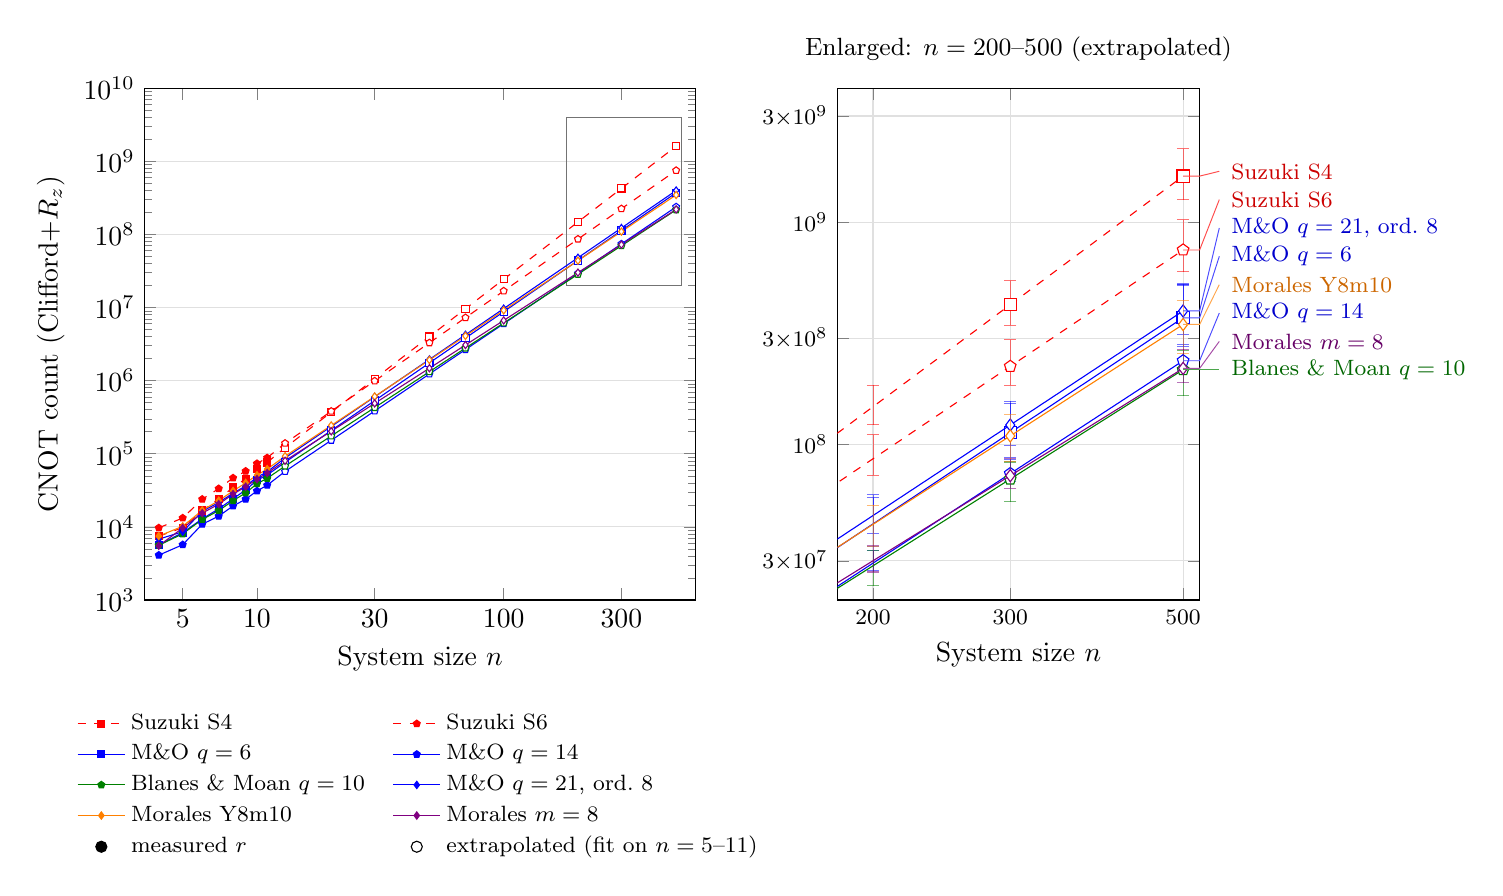
\begin{tikzpicture}
  \begin{loglogaxis}[
    name=main, scale only axis,
    width=7.0cm, height=6.5cm,
    xlabel={System size $n$},
    ylabel={CNOT count (Clifford+$R_z$)},
    xtick={5,10,30,100,300}, xticklabels={5,10,30,100,300},
    xmin=3.5, xmax=600, ymin=1000, ymax=1e+10,
    ymajorgrids=true, grid style={black!12},
    legend style={at={(0.5,-0.2)}, anchor=north, draw=none, font=\footnotesize,
      legend columns=2, /tikz/every even column/.append style={column sep=8pt}},
    legend cell align=left,
  ]
    \draw[black!55, line width=0.5pt] (axis cs:180,2e+07) rectangle (axis cs:525,4e+09);
    \addplot[red, dashed, mark=square*, mark size=1.3pt, mark options={solid, fill=red}] coordinates {
      (4,7459.2)
      (5,9744)
      (6,16707.6)
      (7,24284.4)
      (8,34540.8)
      (9,45549)
      (10,62412)
      (11,76230)
    };
    \addlegendentry{Suzuki S4}
    \addplot[red, dashed, mark=square*, mark size=1.3pt, mark options={solid, fill=white}, mark indices={2,...,10}, forget plot] coordinates {
      (11,76230)
      (13,120830)
      (20,370020)
      (30,1.06155e+06)
      (50,4.00848e+06)
      (70,9.61968e+06)
      (100,2.43394e+07)
      (200,1.47922e+08)
      (300,4.25239e+08)
      (500,1.60899e+09)
    };
    \addplot[red, dashed, mark=pentagon*, mark size=1.3pt, mark options={solid, fill=red}] coordinates {
      (4,9696)
      (5,13231)
      (6,23876.4)
      (7,33370.4)
      (8,46702.4)
      (9,57812.4)
      (10,73528)
      (11,87991.2)
    };
    \addlegendentry{Suzuki S6}
    \addplot[red, dashed, mark=pentagon*, mark size=1.3pt, mark options={solid, fill=white}, mark indices={2,...,10}, forget plot] coordinates {
      (11,87991.2)
      (13,139178)
      (20,381780)
      (30,989598)
      (50,3.2926e+06)
      (70,7.26796e+06)
      (100,1.68428e+07)
      (200,8.62823e+07)
      (300,2.24481e+08)
      (500,7.49087e+08)
    };
    \addplot[blue, solid, mark=square*, mark size=1.3pt, mark options={solid, fill=blue}] coordinates {
      (4,5660)
      (5,8350)
      (6,12870)
      (7,17675)
      (8,24160)
      (9,32085)
      (10,43300)
      (11,51260)
    };
    \addlegendentry{M\&O $q=6$}
    \addplot[blue, solid, mark=square*, mark size=1.3pt, mark options={solid, fill=white}, mark indices={2,...,10}, forget plot] coordinates {
      (11,51260)
      (13,76505)
      (20,207900)
      (30,533100)
      (50,1.74725e+06)
      (70,3.82165e+06)
      (100,8.761e+06)
      (200,4.3965e+07)
      (300,1.13001e+08)
      (500,3.71342e+08)
    };
    \addplot[blue, solid, mark=pentagon*, mark size=1.3pt, mark options={solid, fill=blue}] coordinates {
      (4,4104)
      (5,5700)
      (6,10875.6)
      (7,14044.8)
      (8,19334.4)
      (9,23905.8)
      (10,31008)
      (11,37118.4)
    };
    \addlegendentry{M\&O $q=14$}
    \addplot[blue, solid, mark=pentagon*, mark size=1.3pt, mark options={solid, fill=white}, mark indices={2,...,10}, forget plot] coordinates {
      (11,37118.4)
      (13,57353.4)
      (20,152760)
      (30,384750)
      (50,1.23348e+06)
      (70,2.65973e+06)
      (100,6.00438e+06)
      (200,2.92889e+07)
      (300,7.40054e+07)
      (500,2.37981e+08)
    };
    \addplot[green!50!black, solid, mark=pentagon*, mark size=1.3pt, mark options={solid, fill=green!50!black}] coordinates {
      (4,5608.8)
      (5,8036)
      (6,12644.4)
      (7,16703.4)
      (8,22828.8)
      (9,29151)
      (10,38868)
      (11,46182.4)
    };
    \addlegendentry{Blanes \& Moan $q=10$}
    \addplot[green!50!black, solid, mark=pentagon*, mark size=1.3pt, mark options={solid, fill=white}, mark indices={2,...,10}, forget plot] coordinates {
      (11,46182.4)
      (13,67904.2)
      (20,175152)
      (30,428532)
      (50,1.32553e+06)
      (70,2.78964e+06)
      (100,6.1418e+06)
      (200,2.84934e+07)
      (300,6.99427e+07)
      (500,2.16874e+08)
    };
    \addplot[blue, solid, mark=diamond*, mark size=1.3pt, mark options={solid, fill=blue}] coordinates {
      (4,6800)
      (5,8585)
      (6,16320)
      (7,21539)
      (8,28968)
      (9,36261)
      (10,47770)
      (11,56661)
    };
    \addlegendentry{M\&O $q=21$, ord.~8}
    \addplot[blue, solid, mark=diamond*, mark size=1.3pt, mark options={solid, fill=white}, mark indices={2,...,10}, forget plot] coordinates {
      (11,56661)
      (13,87737)
      (20,236300)
      (30,601290)
      (50,1.95245e+06)
      (70,4.24235e+06)
      (100,9.6662e+06)
      (200,4.79366e+07)
      (300,1.22364e+08)
      (500,3.98548e+08)
    };
    \addplot[orange, solid, mark=diamond*, mark size=1.3pt, mark options={solid, fill=orange}] coordinates {
      (4,7480)
      (5,10200)
      (6,16830)
      (7,22848)
      (8,31008)
      (9,39933)
      (10,51000)
      (11,61710)
    };
    \addlegendentry{Morales Y8m10}
    \addplot[orange, solid, mark=diamond*, mark size=1.3pt, mark options={solid, fill=white}, mark indices={2,...,10}, forget plot] coordinates {
      (11,61710)
      (13,92599)
      (20,244120)
      (30,607410)
      (50,1.9176e+06)
      (70,4.09836e+06)
      (100,9.1596e+06)
      (200,4.3758e+07)
      (300,1.09303e+08)
      (500,3.46477e+08)
    };
    \addplot[violet, solid, mark=diamond*, mark size=1.3pt, mark options={solid, fill=violet}] coordinates {
      (4,5520)
      (5,9660)
      (6,15400.8)
      (7,20479.2)
      (8,28041.6)
      (9,35397)
      (10,44988)
      (11,54496.2)
    };
    \addlegendentry{Morales $m=8$}
    \addplot[violet, solid, mark=diamond*, mark size=1.3pt, mark options={solid, fill=white}, mark indices={2,...,10}, forget plot] coordinates {
      (11,54496.2)
      (13,80191.8)
      (20,203136)
      (30,488934)
      (50,1.47936e+06)
      (70,3.07188e+06)
      (100,6.66264e+06)
      (200,3.0026e+07)
      (300,7.24417e+07)
      (500,2.19834e+08)
    };
    \addlegendimage{only marks, black, mark=*, mark options={solid, fill=black}}
    \addlegendentry{measured $r$}
    \addlegendimage{only marks, black, mark=*, mark options={solid, fill=white}}
    \addlegendentry{extrapolated (fit on $n = 5$--$11$)}
  \end{loglogaxis}
  \begin{loglogaxis}[
    scale only axis,
    at={(8.8cm,0cm)}, anchor=south west,
    width=4.6cm, height=6.5cm,
    title={Enlarged: $n = 200$--$500$ (extrapolated)}, title style={font=\small},
    xlabel={System size $n$},
    xtick={200,300,500}, xticklabels={200,300,500}, xminorticks=false,
    ytick={3e+07,1e+08,3e+08,1e+09,3e+09}, yticklabels={{$3{\times}10^{7}$},{$10^{8}$},{$3{\times}10^{8}$},{$10^{9}$},{$3{\times}10^{9}$}}, yminorticks=false,
    xmin=180, xmax=525, ymin=2e+07, ymax=4e+09,
    xmajorgrids=true, ymajorgrids=true, grid style={black!12}, tick label style={font=\footnotesize},
    clip mode=individual,
  ]
    \addplot[red, dashed, mark=square*, mark size=2.2pt, mark options={solid, fill=white}, mark indices={2,...,10}, forget plot, error bars/.cd, y dir=both, y explicit, error bar style={solid, line width=0.35pt, opacity=0.55}] coordinates {
      (11,76230)
      (13,120830) += (0,5296.2) -= (0,3985.8)
      (20,370020) += (0,27300) -= (0,20580)
      (30,1.06155e+06) += (0,108990) -= (0,81270)
      (50,4.00848e+06) += (0,567420) -= (0,411180)
      (70,9.61968e+06) += (0,1.61112e+06) -= (0,1.14954e+06)
      (100,2.43394e+07) += (0,4.75398e+06) -= (0,3.34362e+06)
      (200,1.47922e+08) += (0,3.70709e+07) -= (0,2.53495e+07)
      (300,4.25239e+08) += (0,1.20644e+08) -= (0,8.11705e+07)
      (500,1.60899e+09) += (0,5.24758e+08) -= (0,3.46154e+08)
    };
    \addplot[red, dashed, mark=pentagon*, mark size=2.2pt, mark options={solid, fill=white}, mark indices={2,...,10}, forget plot, error bars/.cd, y dir=both, y explicit, error bar style={solid, line width=0.35pt, opacity=0.55}] coordinates {
      (11,87991.2)
      (13,139178) += (0,7878) -= (0,2626)
      (20,381780) += (0,30300) -= (0,14140)
      (30,989598) += (0,113322) -= (0,56358)
      (50,3.2926e+06) += (0,525200) -= (0,282800)
      (70,7.26796e+06) += (0,1.37158e+06) -= (0,749420)
      (100,1.68428e+07) += (0,3.70064e+06) -= (0,2.03616e+06)
      (200,8.62823e+07) += (0,2.43733e+07) -= (0,1.34411e+07)
      (300,2.24481e+08) += (0,7.17928e+07) -= (0,3.94688e+07)
      (500,7.49087e+08) += (0,2.75659e+08) -= (0,1.50258e+08)
    };
    \addplot[blue, solid, mark=square*, mark size=2.2pt, mark options={solid, fill=white}, mark indices={2,...,10}, forget plot, error bars/.cd, y dir=both, y explicit, error bar style={solid, line width=0.35pt, opacity=0.55}] coordinates {
      (11,51260)
      (13,76505) += (0,4745) -= (0,3055)
      (20,207900) += (0,21100) -= (0,12900)
      (30,533100) += (0,72900) -= (0,48600)
      (50,1.74725e+06) += (0,320250) -= (0,214750)
      (70,3.82165e+06) += (0,815850) -= (0,545650)
      (100,8.761e+06) += (0,2.164e+06) -= (0,1.441e+06)
      (200,4.3965e+07) += (0,1.3765e+07) -= (0,9.035e+06)
      (300,1.13001e+08) += (0,3.9894e+07) -= (0,2.5851e+07)
      (500,3.71342e+08) += (0,1.50232e+08) -= (0,9.55425e+07)
    };
    \addplot[blue, solid, mark=pentagon*, mark size=2.2pt, mark options={solid, fill=white}, mark indices={2,...,10}, forget plot, error bars/.cd, y dir=both, y explicit, error bar style={solid, line width=0.35pt, opacity=0.55}] coordinates {
      (11,37118.4)
      (13,57353.4) += (0,444.6) -= (0,1037.4)
      (20,152760) += (0,4560) -= (0,4560)
      (30,384750) += (0,18810) -= (0,15390)
      (50,1.23348e+06) += (0,88920) -= (0,59280)
      (70,2.65973e+06) += (0,237006) -= (0,146034)
      (100,6.00438e+06) += (0,641820) -= (0,361380)
      (200,2.92889e+07) += (0,4.09032e+06) -= (0,2.15688e+06)
      (300,7.40054e+07) += (0,1.18366e+07) -= (0,6.04998e+06)
      (500,2.37981e+08) += (0,4.40553e+07) -= (0,2.17797e+07)
    };
    \addplot[green!50!black, solid, mark=pentagon*, mark size=2.2pt, mark options={solid, fill=white}, mark indices={2,...,10}, forget plot, error bars/.cd, y dir=both, y explicit, error bar style={solid, line width=0.35pt, opacity=0.55}] coordinates {
      (11,46182.4)
      (13,67904.2) += (0,1385.8) -= (0,1812.2)
      (20,175152) += (0,6888) -= (0,9512)
      (30,428532) += (0,26568) -= (0,34932)
      (50,1.32553e+06) += (0,121770) -= (0,144730)
      (70,2.78964e+06) += (0,304220) -= (0,361620)
      (100,6.1418e+06) += (0,795400) -= (0,918400)
      (200,2.84934e+07) += (0,4.83144e+06) -= (0,5.33656e+06)
      (300,6.99427e+07) += (0,1.34759e+07) -= (0,1.45927e+07)
      (500,2.16874e+08) += (0,4.82324e+07) -= (0,5.09876e+07)
    };
    \addplot[blue, solid, mark=diamond*, mark size=2.2pt, mark options={solid, fill=white}, mark indices={2,...,10}, forget plot, error bars/.cd, y dir=both, y explicit, error bar style={solid, line width=0.35pt, opacity=0.55}] coordinates {
      (11,56661)
      (13,87737) += (0,2873) -= (0,1547)
      (20,236300) += (0,15300) -= (0,8500)
      (30,601290) += (0,51510) -= (0,35190)
      (50,1.95245e+06) += (0,249050) -= (0,175950)
      (70,4.24235e+06) += (0,660450) -= (0,458150)
      (100,9.6662e+06) += (0,1.7918e+06) -= (0,1.2512e+06)
      (200,4.79366e+07) += (0,1.16314e+07) -= (0,8.0206e+06)
      (300,1.22364e+08) += (0,3.39507e+07) -= (0,2.30673e+07)
      (500,3.98548e+08) += (0,1.28537e+08) -= (0,8.5833e+07)
    };
    \addplot[orange, solid, mark=diamond*, mark size=2.2pt, mark options={solid, fill=white}, mark indices={2,...,10}, forget plot, error bars/.cd, y dir=both, y explicit, error bar style={solid, line width=0.35pt, opacity=0.55}] coordinates {
      (11,61710)
      (13,92599) += (0,2431) -= (0,4199)
      (20,244120) += (0,14280) -= (0,16320)
      (30,607410) += (0,55590) -= (0,56610)
      (50,1.9176e+06) += (0,232900) -= (0,243100)
      (70,4.09836e+06) += (0,590240) -= (0,599760)
      (100,9.1596e+06) += (0,1.5504e+06) -= (0,1.5436e+06)
      (200,4.3758e+07) += (0,9.554e+06) -= (0,9.112e+06)
      (300,1.09303e+08) += (0,2.70198e+07) -= (0,2.52552e+07)
      (500,3.46477e+08) += (0,9.8413e+07) -= (0,8.9862e+07)
    };
    \addplot[violet, solid, mark=diamond*, mark size=2.2pt, mark options={solid, fill=white}, mark indices={2,...,10}, forget plot, error bars/.cd, y dir=both, y explicit, error bar style={solid, line width=0.35pt, opacity=0.55}] coordinates {
      (11,54496.2)
      (13,80191.8) += (0,2332.2) -= (0,1255.8)
      (20,203136) += (0,9384) -= (0,7176)
      (30,488934) += (0,32706) -= (0,25254)
      (50,1.47936e+06) += (0,142140) -= (0,99360)
      (70,3.07188e+06) += (0,338100) -= (0,231840)
      (100,6.66264e+06) += (0,872160) -= (0,590640)
      (200,3.0026e+07) += (0,5.02596e+06) -= (0,3.30924e+06)
      (300,7.24417e+07) += (0,1.37117e+07) -= (0,8.89272e+06)
      (500,2.19834e+08) += (0,4.7817e+07) -= (0,3.0498e+07)
    };
    \draw[red!70, line width=0.35pt] (axis cs:500,1.60899e+09) -- (axis cs:525,1.60899e+09) -- ([xshift=0.25cm]axis cs:525,1.69161e+09);
    \node[anchor=west, font=\footnotesize, text=red!80!black] at ([xshift=0.28cm]axis cs:525,1.69161e+09) {Suzuki S4};
    \draw[red!70, line width=0.35pt] (axis cs:500,7.49087e+08) -- (axis cs:525,7.49087e+08) -- ([xshift=0.25cm]axis cs:525,1.26141e+09);
    \node[anchor=west, font=\footnotesize, text=red!80!black] at ([xshift=0.28cm]axis cs:525,1.26141e+09) {Suzuki S6};
    \draw[blue!70, line width=0.35pt] (axis cs:500,3.71342e+08) -- (axis cs:525,3.71342e+08) -- ([xshift=0.25cm]axis cs:525,7.01414e+08);
    \node[anchor=west, font=\footnotesize, text=blue!80!black] at ([xshift=0.28cm]axis cs:525,7.01414e+08) {M\&O $q=6$};
    \draw[blue!70, line width=0.35pt] (axis cs:500,2.37981e+08) -- (axis cs:525,2.37981e+08) -- ([xshift=0.25cm]axis cs:525,3.90024e+08);
    \node[anchor=west, font=\footnotesize, text=blue!80!black] at ([xshift=0.28cm]axis cs:525,3.90024e+08) {M\&O $q=14$};
    \draw[green!50!black!70, line width=0.35pt] (axis cs:500,2.16874e+08) -- (axis cs:525,2.16874e+08) -- ([xshift=0.25cm]axis cs:525,2.16874e+08);
    \node[anchor=west, font=\footnotesize, text=green!50!black!80!black] at ([xshift=0.28cm]axis cs:525,2.16874e+08) {Blanes \& Moan $q=10$};
    \draw[blue!70, line width=0.35pt] (axis cs:500,3.98548e+08) -- (axis cs:525,3.98548e+08) -- ([xshift=0.25cm]axis cs:525,9.40623e+08);
    \node[anchor=west, font=\footnotesize, text=blue!80!black] at ([xshift=0.28cm]axis cs:525,9.40623e+08) {M\&O $q=21$, ord.~8};
    \draw[orange!70, line width=0.35pt] (axis cs:500,3.46477e+08) -- (axis cs:525,3.46477e+08) -- ([xshift=0.25cm]axis cs:525,5.23037e+08);
    \node[anchor=west, font=\footnotesize, text=orange!80!black] at ([xshift=0.28cm]axis cs:525,5.23037e+08) {Morales Y8m10};
    \draw[violet!70, line width=0.35pt] (axis cs:500,2.19834e+08) -- (axis cs:525,2.19834e+08) -- ([xshift=0.25cm]axis cs:525,2.90837e+08);
    \node[anchor=west, font=\footnotesize, text=violet!80!black] at ([xshift=0.28cm]axis cs:525,2.90837e+08) {Morales $m=8$};
  \end{loglogaxis}
\end{tikzpicture}
  \end{fitwidth}\par\bigskip
  \begin{fitwidth}
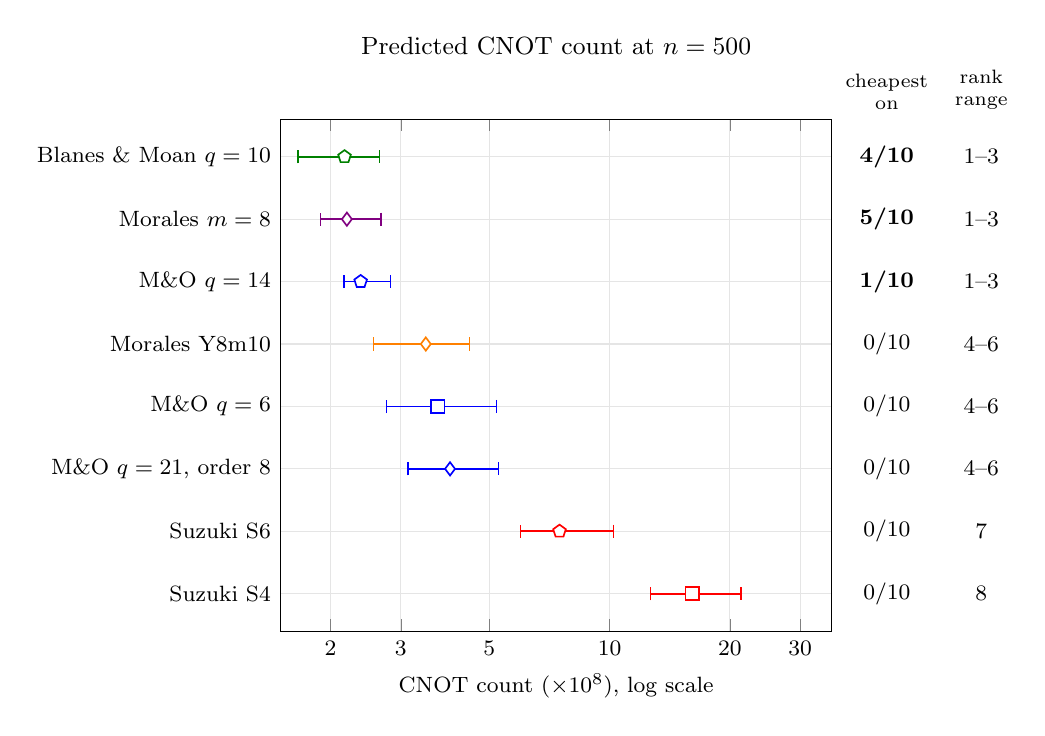
\begin{tikzpicture}
  \begin{semilogxaxis}[
    scale only axis, clip=false,
    at={(0cm,0cm)}, anchor=south west,
    width=7.0cm, height=6.5cm,
    title={Predicted CNOT count at $n = 500$}, title style={font=\small, yshift=14pt},
    xlabel={CNOT count ($\times 10^{8}$), log scale}, xlabel style={font=\footnotesize},
    xmin=1.5e+08, xmax=3.6e+09, xtick={2e+08,3e+08,5e+08,1e+09,2e+09,3e+09}, xticklabels={2,3,5,10,20,30},
    xminorticks=false,
    y dir=reverse, ymin=0.4, ymax=8.6, ytick={1,2,3,4,5,6,7,8},
    yticklabels={{Blanes \& Moan $q=10$},{Morales $m=8$},{M\&O $q=14$},{Morales Y8m10},{M\&O $q=6$},{M\&O $q=21$, order 8},{Suzuki S6},{Suzuki S4}},
    tick label style={font=\footnotesize}, ytick style={draw=none},
    xmajorgrids=true, ymajorgrids=true, grid style={black!10},
  ]
    \addplot[green!50!black, only marks, mark=pentagon*, mark size=2.4pt, mark options={solid, fill=white, line width=0.6pt}, error bars/.cd, x dir=both, x explicit, error bar style={solid, line width=0.6pt}] coordinates {
      (2.16874e+08,1) += (4.82324e+07,0) -= (5.09876e+07,0)
    };
    \addplot[violet, only marks, mark=diamond*, mark size=2.4pt, mark options={solid, fill=white, line width=0.6pt}, error bars/.cd, x dir=both, x explicit, error bar style={solid, line width=0.6pt}] coordinates {
      (2.19834e+08,2) += (4.7817e+07,0) -= (3.0498e+07,0)
    };
    \addplot[blue, only marks, mark=pentagon*, mark size=2.4pt, mark options={solid, fill=white, line width=0.6pt}, error bars/.cd, x dir=both, x explicit, error bar style={solid, line width=0.6pt}] coordinates {
      (2.37981e+08,3) += (4.40553e+07,0) -= (2.17797e+07,0)
    };
    \addplot[orange, only marks, mark=diamond*, mark size=2.4pt, mark options={solid, fill=white, line width=0.6pt}, error bars/.cd, x dir=both, x explicit, error bar style={solid, line width=0.6pt}] coordinates {
      (3.46477e+08,4) += (9.8413e+07,0) -= (8.9862e+07,0)
    };
    \addplot[blue, only marks, mark=square*, mark size=2.4pt, mark options={solid, fill=white, line width=0.6pt}, error bars/.cd, x dir=both, x explicit, error bar style={solid, line width=0.6pt}] coordinates {
      (3.71342e+08,5) += (1.50232e+08,0) -= (9.55425e+07,0)
    };
    \addplot[blue, only marks, mark=diamond*, mark size=2.4pt, mark options={solid, fill=white, line width=0.6pt}, error bars/.cd, x dir=both, x explicit, error bar style={solid, line width=0.6pt}] coordinates {
      (3.98548e+08,6) += (1.28537e+08,0) -= (8.5833e+07,0)
    };
    \addplot[red, only marks, mark=pentagon*, mark size=2.4pt, mark options={solid, fill=white, line width=0.6pt}, error bars/.cd, x dir=both, x explicit, error bar style={solid, line width=0.6pt}] coordinates {
      (7.49087e+08,7) += (2.75659e+08,0) -= (1.50258e+08,0)
    };
    \addplot[red, only marks, mark=square*, mark size=2.4pt, mark options={solid, fill=white, line width=0.6pt}, error bars/.cd, x dir=both, x explicit, error bar style={solid, line width=0.6pt}] coordinates {
      (1.60899e+09,8) += (5.24758e+08,0) -= (3.46154e+08,0)
    };
    \node[anchor=south, font=\scriptsize, align=center] at ([xshift=0.7cm]axis cs:3.6e+09,0.4) {cheapest\\on};
    \node[anchor=south, font=\scriptsize, align=center] at ([xshift=1.9cm]axis cs:3.6e+09,0.4) {rank\\range};
    \node[font=\footnotesize\bfseries] at ([xshift=0.7cm]axis cs:3.6e+09,1) {4/10};
    \node[font=\footnotesize] at ([xshift=1.9cm]axis cs:3.6e+09,1) {1--3};
    \node[font=\footnotesize\bfseries] at ([xshift=0.7cm]axis cs:3.6e+09,2) {5/10};
    \node[font=\footnotesize] at ([xshift=1.9cm]axis cs:3.6e+09,2) {1--3};
    \node[font=\footnotesize\bfseries] at ([xshift=0.7cm]axis cs:3.6e+09,3) {1/10};
    \node[font=\footnotesize] at ([xshift=1.9cm]axis cs:3.6e+09,3) {1--3};
    \node[font=\footnotesize] at ([xshift=0.7cm]axis cs:3.6e+09,4) {0/10};
    \node[font=\footnotesize] at ([xshift=1.9cm]axis cs:3.6e+09,4) {4--6};
    \node[font=\footnotesize] at ([xshift=0.7cm]axis cs:3.6e+09,5) {0/10};
    \node[font=\footnotesize] at ([xshift=1.9cm]axis cs:3.6e+09,5) {4--6};
    \node[font=\footnotesize] at ([xshift=0.7cm]axis cs:3.6e+09,6) {0/10};
    \node[font=\footnotesize] at ([xshift=1.9cm]axis cs:3.6e+09,6) {4--6};
    \node[font=\footnotesize] at ([xshift=0.7cm]axis cs:3.6e+09,7) {0/10};
    \node[font=\footnotesize] at ([xshift=1.9cm]axis cs:3.6e+09,7) {7};
    \node[font=\footnotesize] at ([xshift=0.7cm]axis cs:3.6e+09,8) {0/10};
    \node[font=\footnotesize] at ([xshift=1.9cm]axis cs:3.6e+09,8) {8};
  \end{semilogxaxis}
\end{tikzpicture}
  \end{fitwidth}
    \caption{CNOT count against system size, extrapolated to $n = 500$: full range and $n = 200$--$500$ enlarged (top); predicted count at $n = 500$ over seeds (bottom)}
\end{figure}
\clearpage
\pagelabel{2}{CNOT count}{Minimised bound $r$}{norm bound evaluated at every $n = 4$--$500$}{New; counterpart of Figure~4.3}
\begin{figure}[H]
  \centering
  \begin{fitwidth}
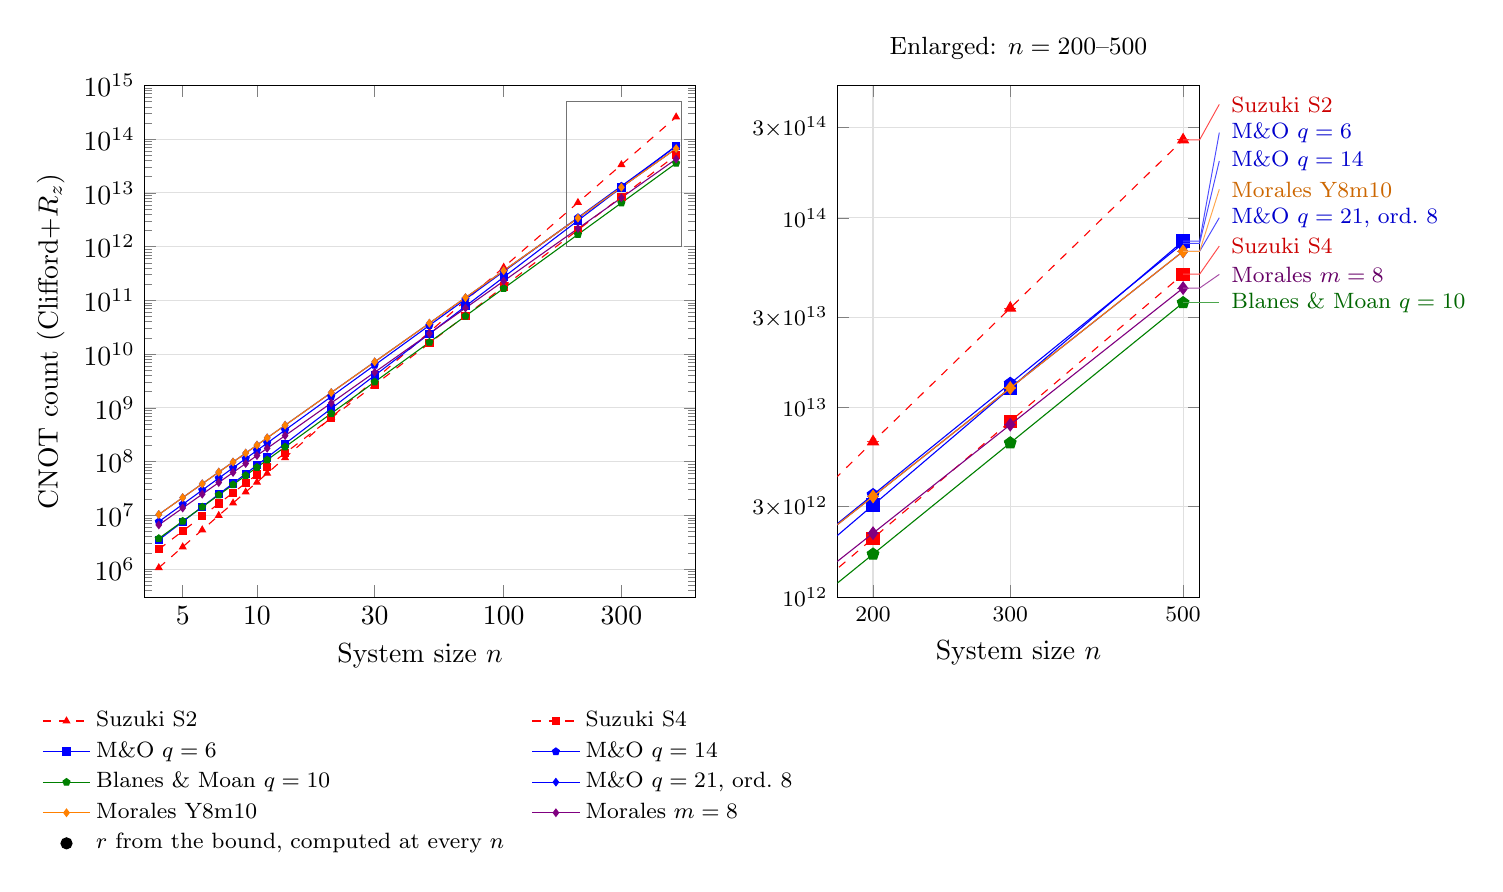
\begin{tikzpicture}
  \begin{loglogaxis}[
    name=main, scale only axis,
    width=7.0cm, height=6.5cm,
    xlabel={System size $n$},
    ylabel={CNOT count (Clifford+$R_z$)},
    xtick={5,10,30,100,300}, xticklabels={5,10,30,100,300},
    xmin=3.5, xmax=600, ymin=300000, ymax=1e+15,
    ymajorgrids=true, grid style={black!12},
    legend style={at={(0.5,-0.2)}, anchor=north, draw=none, font=\footnotesize,
      legend columns=2, /tikz/every even column/.append style={column sep=8pt}},
    legend cell align=left,
  ]
    \draw[black!55, line width=0.5pt] (axis cs:180,1e+12) rectangle (axis cs:525,5e+14);
    \addplot[red, dashed, mark=triangle*, mark size=1.3pt, mark options={solid, fill=red}] coordinates {
      (4,1.06016e+06)
      (5,2.587e+06)
      (6,5.36268e+06)
      (7,9.93272e+06)
      (8,1.69418e+07)
      (9,2.71339e+07)
      (10,4.13519e+07)
      (11,6.0538e+07)
      (13,1.18079e+08)
      (20,6.61309e+08)
      (30,3.34734e+09)
      (50,2.58249e+10)
      (70,9.92034e+10)
      (100,4.13158e+11)
      (200,6.61021e+12)
      (300,3.34637e+13)
      (500,2.58204e+14)
    };
    \addlegendentry{Suzuki S2}
    \addplot[red, dashed, mark=square*, mark size=1.3pt, mark options={solid, fill=red}] coordinates {
      (4,2.33755e+06)
      (5,5.09817e+06)
      (6,9.64202e+06)
      (7,1.65263e+07)
      (8,2.63575e+07)
      (9,3.97868e+07)
      (10,5.75064e+07)
      (11,8.02499e+07)
      (13,1.43923e+08)
      (20,6.49228e+08)
      (30,2.68105e+09)
      (50,1.6009e+10)
      (70,5.19507e+10)
      (100,1.80947e+11)
      (200,2.0458e+12)
      (300,8.45378e+12)
      (500,5.05115e+13)
    };
    \addlegendentry{Suzuki S4}
    \addplot[blue, solid, mark=square*, mark size=1.3pt, mark options={solid, fill=blue}] coordinates {
      (4,3.4934e+06)
      (5,7.61925e+06)
      (6,1.44105e+07)
      (7,2.47006e+07)
      (8,3.93952e+07)
      (9,5.94684e+07)
      (10,8.59555e+07)
      (11,1.19952e+08)
      (13,2.15132e+08)
      (20,9.70498e+08)
      (30,4.00794e+09)
      (50,2.3933e+10)
      (70,7.76668e+10)
      (100,2.70523e+11)
      (200,3.05864e+12)
      (300,1.26393e+13)
      (500,7.5521e+13)
    };
    \addlegendentry{M\&O $q=6$}
    \addplot[blue, solid, mark=pentagon*, mark size=1.3pt, mark options={solid, fill=blue}] coordinates {
      (4,7.63435e+06)
      (5,1.60415e+07)
      (6,2.94284e+07)
      (7,4.91568e+07)
      (8,7.66682e+07)
      (9,1.13471e+08)
      (10,1.61142e+08)
      (11,2.21313e+08)
      (13,3.85962e+08)
      (20,1.61983e+09)
      (30,6.24984e+09)
      (50,3.42566e+10)
      (70,1.05071e+11)
      (100,3.44736e+11)
      (200,3.47032e+12)
      (300,1.3399e+13)
      (500,7.34983e+13)
    };
    \addlegendentry{M\&O $q=14$}
    \addplot[green!50!black, solid, mark=pentagon*, mark size=1.3pt, mark options={solid, fill=green!50!black}] coordinates {
      (4,3.7123e+06)
      (5,7.79984e+06)
      (6,1.43079e+07)
      (7,2.38991e+07)
      (8,3.72726e+07)
      (9,5.51633e+07)
      (10,7.83362e+07)
      (11,1.07585e+08)
      (13,1.87617e+08)
      (20,7.87331e+08)
      (30,3.03755e+09)
      (50,1.66481e+10)
      (70,5.10601e+10)
      (100,1.6752e+11)
      (200,1.68623e+12)
      (300,6.51037e+12)
      (500,3.57103e+13)
    };
    \addlegendentry{Blanes \& Moan $q=10$}
    \addplot[blue, solid, mark=diamond*, mark size=1.3pt, mark options={solid, fill=blue}] coordinates {
      (4,1.03646e+07)
      (5,2.138e+07)
      (6,3.86325e+07)
      (7,6.3709e+07)
      (8,9.82668e+07)
      (9,1.44019e+08)
      (10,2.02737e+08)
      (11,2.76236e+08)
      (13,4.75081e+08)
      (20,1.92344e+09)
      (30,7.174e+09)
      (50,3.76772e+10)
      (70,1.12353e+11)
      (100,3.57779e+11)
      (200,3.39843e+12)
      (300,1.26831e+13)
      (500,6.66564e+13)
    };
    \addlegendentry{M\&O $q=21$, ord.~8}
    \addplot[orange, solid, mark=diamond*, mark size=1.3pt, mark options={solid, fill=orange}] coordinates {
      (4,1.03646e+07)
      (5,2.138e+07)
      (6,3.86325e+07)
      (7,6.3709e+07)
      (8,9.82668e+07)
      (9,1.44019e+08)
      (10,2.02737e+08)
      (11,2.76236e+08)
      (13,4.75081e+08)
      (20,1.92344e+09)
      (30,7.174e+09)
      (50,3.76772e+10)
      (70,1.12353e+11)
      (100,3.57779e+11)
      (200,3.39843e+12)
      (300,1.26831e+13)
      (500,6.66564e+13)
    };
    \addlegendentry{Morales Y8m10}
    \addplot[violet, solid, mark=diamond*, mark size=1.3pt, mark options={solid, fill=violet}] coordinates {
      (4,6.6378e+06)
      (5,1.3691e+07)
      (6,2.47382e+07)
      (7,4.07951e+07)
      (8,6.29225e+07)
      (9,9.22185e+07)
      (10,1.29814e+08)
      (11,1.76874e+08)
      (13,3.04191e+08)
      (20,1.23151e+09)
      (30,4.59308e+09)
      (50,2.41214e+10)
      (70,7.19279e+10)
      (100,2.29044e+11)
      (200,2.17553e+12)
      (300,8.119e+12)
      (500,4.26685e+13)
    };
    \addlegendentry{Morales $m=8$}
    \addlegendimage{only marks, black, mark=*, mark options={solid, fill=black}}
    \addlegendentry{$r$ from the bound, computed at every $n$}
  \end{loglogaxis}
  \begin{loglogaxis}[
    scale only axis,
    at={(8.8cm,0cm)}, anchor=south west,
    width=4.6cm, height=6.5cm,
    title={Enlarged: $n = 200$--$500$}, title style={font=\small},
    xlabel={System size $n$},
    xtick={200,300,500}, xticklabels={200,300,500}, xminorticks=false,
    ytick={1e+12,3e+12,1e+13,3e+13,1e+14,3e+14}, yticklabels={{$10^{12}$},{$3{\times}10^{12}$},{$10^{13}$},{$3{\times}10^{13}$},{$10^{14}$},{$3{\times}10^{14}$}}, yminorticks=false,
    xmin=180, xmax=525, ymin=1e+12, ymax=5e+14,
    xmajorgrids=true, ymajorgrids=true, grid style={black!12}, tick label style={font=\footnotesize},
    clip mode=individual,
  ]
    \addplot[red, dashed, mark=triangle*, mark size=2.2pt, mark options={solid, fill=red}, forget plot, error bars/.cd, y dir=both, y explicit, error bar style={solid, line width=0.35pt, opacity=0.55}] coordinates {
      (4,1.06016e+06) += (0,0) -= (0,0)
      (5,2.587e+06) += (0,0) -= (0,0)
      (6,5.36268e+06) += (0,0) -= (0,0)
      (7,9.93272e+06) += (0,0) -= (0,0)
      (8,1.69418e+07) += (0,0) -= (0,0)
      (9,2.71339e+07) += (0,0) -= (0,0)
      (10,4.13519e+07) += (0,0) -= (0,0)
      (11,6.0538e+07) += (0,0) -= (0,0)
      (13,1.18079e+08) += (0,0) -= (0,0)
      (20,6.61309e+08) += (0,0) -= (0,0)
      (30,3.34734e+09) += (0,0) -= (0,0)
      (50,2.58249e+10) += (0,0) -= (0,0)
      (70,9.92034e+10) += (0,0) -= (0,0)
      (100,4.13158e+11) += (0,0) -= (0,0)
      (200,6.61021e+12) += (0,0) -= (0,0)
      (300,3.34637e+13) += (0,0) -= (0,0)
      (500,2.58204e+14) += (0,0) -= (0,0)
    };
    \addplot[red, dashed, mark=square*, mark size=2.2pt, mark options={solid, fill=red}, forget plot, error bars/.cd, y dir=both, y explicit, error bar style={solid, line width=0.35pt, opacity=0.55}] coordinates {
      (4,2.33755e+06) += (0,0) -= (0,0)
      (5,5.09817e+06) += (0,0) -= (0,0)
      (6,9.64202e+06) += (0,0) -= (0,0)
      (7,1.65263e+07) += (0,0) -= (0,0)
      (8,2.63575e+07) += (0,0) -= (0,0)
      (9,3.97868e+07) += (0,0) -= (0,0)
      (10,5.75064e+07) += (0,0) -= (0,0)
      (11,8.02499e+07) += (0,0) -= (0,0)
      (13,1.43923e+08) += (0,0) -= (0,0)
      (20,6.49228e+08) += (0,0) -= (0,0)
      (30,2.68105e+09) += (0,0) -= (0,0)
      (50,1.6009e+10) += (0,0) -= (0,0)
      (70,5.19507e+10) += (0,0) -= (0,0)
      (100,1.80947e+11) += (0,0) -= (0,0)
      (200,2.0458e+12) += (0,0) -= (0,0)
      (300,8.45378e+12) += (0,0) -= (0,0)
      (500,5.05115e+13) += (0,0) -= (0,0)
    };
    \addplot[blue, solid, mark=square*, mark size=2.2pt, mark options={solid, fill=blue}, forget plot, error bars/.cd, y dir=both, y explicit, error bar style={solid, line width=0.35pt, opacity=0.55}] coordinates {
      (4,3.4934e+06) += (0,0) -= (0,0)
      (5,7.61925e+06) += (0,0) -= (0,0)
      (6,1.44105e+07) += (0,0) -= (0,0)
      (7,2.47006e+07) += (0,0) -= (0,0)
      (8,3.93952e+07) += (0,0) -= (0,0)
      (9,5.94684e+07) += (0,0) -= (0,0)
      (10,8.59555e+07) += (0,0) -= (0,0)
      (11,1.19952e+08) += (0,0) -= (0,0)
      (13,2.15132e+08) += (0,0) -= (0,0)
      (20,9.70498e+08) += (0,0) -= (0,0)
      (30,4.00794e+09) += (0,0) -= (0,0)
      (50,2.3933e+10) += (0,0) -= (0,0)
      (70,7.76668e+10) += (0,0) -= (0,0)
      (100,2.70523e+11) += (0,0) -= (0,0)
      (200,3.05864e+12) += (0,0) -= (0,0)
      (300,1.26393e+13) += (0,0) -= (0,0)
      (500,7.5521e+13) += (0,0) -= (0,0)
    };
    \addplot[blue, solid, mark=pentagon*, mark size=2.2pt, mark options={solid, fill=blue}, forget plot, error bars/.cd, y dir=both, y explicit, error bar style={solid, line width=0.35pt, opacity=0.55}] coordinates {
      (4,7.63435e+06) += (0,0) -= (0,0)
      (5,1.60415e+07) += (0,0) -= (0,0)
      (6,2.94284e+07) += (0,0) -= (0,0)
      (7,4.91568e+07) += (0,0) -= (0,0)
      (8,7.66682e+07) += (0,0) -= (0,0)
      (9,1.13471e+08) += (0,0) -= (0,0)
      (10,1.61142e+08) += (0,0) -= (0,0)
      (11,2.21313e+08) += (0,0) -= (0,0)
      (13,3.85962e+08) += (0,0) -= (0,0)
      (20,1.61983e+09) += (0,0) -= (0,0)
      (30,6.24984e+09) += (0,0) -= (0,0)
      (50,3.42566e+10) += (0,0) -= (0,0)
      (70,1.05071e+11) += (0,0) -= (0,0)
      (100,3.44736e+11) += (0,0) -= (0,0)
      (200,3.47032e+12) += (0,0) -= (0,0)
      (300,1.3399e+13) += (0,0) -= (0,0)
      (500,7.34983e+13) += (0,0) -= (0,0)
    };
    \addplot[green!50!black, solid, mark=pentagon*, mark size=2.2pt, mark options={solid, fill=green!50!black}, forget plot, error bars/.cd, y dir=both, y explicit, error bar style={solid, line width=0.35pt, opacity=0.55}] coordinates {
      (4,3.7123e+06) += (0,0) -= (0,0)
      (5,7.79984e+06) += (0,0) -= (0,0)
      (6,1.43079e+07) += (0,0) -= (0,0)
      (7,2.38991e+07) += (0,0) -= (0,0)
      (8,3.72726e+07) += (0,0) -= (0,0)
      (9,5.51633e+07) += (0,0) -= (0,0)
      (10,7.83362e+07) += (0,0) -= (0,0)
      (11,1.07585e+08) += (0,0) -= (0,0)
      (13,1.87617e+08) += (0,0) -= (0,0)
      (20,7.87331e+08) += (0,0) -= (0,0)
      (30,3.03755e+09) += (0,0) -= (0,0)
      (50,1.66481e+10) += (0,0) -= (0,0)
      (70,5.10601e+10) += (0,0) -= (0,0)
      (100,1.6752e+11) += (0,0) -= (0,0)
      (200,1.68623e+12) += (0,0) -= (0,0)
      (300,6.51037e+12) += (0,0) -= (0,0)
      (500,3.57103e+13) += (0,0) -= (0,0)
    };
    \addplot[blue, solid, mark=diamond*, mark size=2.2pt, mark options={solid, fill=blue}, forget plot, error bars/.cd, y dir=both, y explicit, error bar style={solid, line width=0.35pt, opacity=0.55}] coordinates {
      (4,1.03646e+07) += (0,0) -= (0,0)
      (5,2.138e+07) += (0,0) -= (0,0)
      (6,3.86325e+07) += (0,0) -= (0,0)
      (7,6.3709e+07) += (0,0) -= (0,0)
      (8,9.82668e+07) += (0,0) -= (0,0)
      (9,1.44019e+08) += (0,0) -= (0,0)
      (10,2.02737e+08) += (0,0) -= (0,0)
      (11,2.76236e+08) += (0,0) -= (0,0)
      (13,4.75081e+08) += (0,0) -= (0,0)
      (20,1.92344e+09) += (0,0) -= (0,0)
      (30,7.174e+09) += (0,0) -= (0,0)
      (50,3.76772e+10) += (0,0) -= (0,0)
      (70,1.12353e+11) += (0,0) -= (0,0)
      (100,3.57779e+11) += (0,0) -= (0,0)
      (200,3.39843e+12) += (0,0) -= (0,0)
      (300,1.26831e+13) += (0,0) -= (0,0)
      (500,6.66564e+13) += (0,0) -= (0,0)
    };
    \addplot[orange, solid, mark=diamond*, mark size=2.2pt, mark options={solid, fill=orange}, forget plot, error bars/.cd, y dir=both, y explicit, error bar style={solid, line width=0.35pt, opacity=0.55}] coordinates {
      (4,1.03646e+07) += (0,0) -= (0,0)
      (5,2.138e+07) += (0,0) -= (0,0)
      (6,3.86325e+07) += (0,0) -= (0,0)
      (7,6.3709e+07) += (0,0) -= (0,0)
      (8,9.82668e+07) += (0,0) -= (0,0)
      (9,1.44019e+08) += (0,0) -= (0,0)
      (10,2.02737e+08) += (0,0) -= (0,0)
      (11,2.76236e+08) += (0,0) -= (0,0)
      (13,4.75081e+08) += (0,0) -= (0,0)
      (20,1.92344e+09) += (0,0) -= (0,0)
      (30,7.174e+09) += (0,0) -= (0,0)
      (50,3.76772e+10) += (0,0) -= (0,0)
      (70,1.12353e+11) += (0,0) -= (0,0)
      (100,3.57779e+11) += (0,0) -= (0,0)
      (200,3.39843e+12) += (0,0) -= (0,0)
      (300,1.26831e+13) += (0,0) -= (0,0)
      (500,6.66564e+13) += (0,0) -= (0,0)
    };
    \addplot[violet, solid, mark=diamond*, mark size=2.2pt, mark options={solid, fill=violet}, forget plot, error bars/.cd, y dir=both, y explicit, error bar style={solid, line width=0.35pt, opacity=0.55}] coordinates {
      (4,6.6378e+06) += (0,0) -= (0,0)
      (5,1.3691e+07) += (0,0) -= (0,0)
      (6,2.47382e+07) += (0,0) -= (0,0)
      (7,4.07951e+07) += (0,0) -= (0,0)
      (8,6.29225e+07) += (0,0) -= (0,0)
      (9,9.22185e+07) += (0,0) -= (0,0)
      (10,1.29814e+08) += (0,0) -= (0,0)
      (11,1.76874e+08) += (0,0) -= (0,0)
      (13,3.04191e+08) += (0,0) -= (0,0)
      (20,1.23151e+09) += (0,0) -= (0,0)
      (30,4.59308e+09) += (0,0) -= (0,0)
      (50,2.41214e+10) += (0,0) -= (0,0)
      (70,7.19279e+10) += (0,0) -= (0,0)
      (100,2.29044e+11) += (0,0) -= (0,0)
      (200,2.17553e+12) += (0,0) -= (0,0)
      (300,8.119e+12) += (0,0) -= (0,0)
      (500,4.26685e+13) += (0,0) -= (0,0)
    };
    \draw[red!70, line width=0.35pt] (axis cs:500,2.58204e+14) -- (axis cs:525,2.58204e+14) -- ([xshift=0.25cm]axis cs:525,3.97341e+14);
    \node[anchor=west, font=\footnotesize, text=red!80!black] at ([xshift=0.28cm]axis cs:525,3.97341e+14) {Suzuki S2};
    \draw[red!70, line width=0.35pt] (axis cs:500,5.05115e+13) -- (axis cs:525,5.05115e+13) -- ([xshift=0.25cm]axis cs:525,7.10815e+13);
    \node[anchor=west, font=\footnotesize, text=red!80!black] at ([xshift=0.28cm]axis cs:525,7.10815e+13) {Suzuki S4};
    \draw[blue!70, line width=0.35pt] (axis cs:500,7.5521e+13) -- (axis cs:525,7.5521e+13) -- ([xshift=0.25cm]axis cs:525,2.81632e+14);
    \node[anchor=west, font=\footnotesize, text=blue!80!black] at ([xshift=0.28cm]axis cs:525,2.81632e+14) {M\&O $q=6$};
    \draw[blue!70, line width=0.35pt] (axis cs:500,7.34983e+13) -- (axis cs:525,7.34983e+13) -- ([xshift=0.25cm]axis cs:525,1.99618e+14);
    \node[anchor=west, font=\footnotesize, text=blue!80!black] at ([xshift=0.28cm]axis cs:525,1.99618e+14) {M\&O $q=14$};
    \draw[green!50!black!70, line width=0.35pt] (axis cs:500,3.57103e+13) -- (axis cs:525,3.57103e+13) -- ([xshift=0.25cm]axis cs:525,3.57103e+13);
    \node[anchor=west, font=\footnotesize, text=green!50!black!80!black] at ([xshift=0.28cm]axis cs:525,3.57103e+13) {Blanes \& Moan $q=10$};
    \draw[blue!70, line width=0.35pt] (axis cs:500,6.66564e+13) -- (axis cs:525,6.66564e+13) -- ([xshift=0.25cm]axis cs:525,1.00285e+14);
    \node[anchor=west, font=\footnotesize, text=blue!80!black] at ([xshift=0.28cm]axis cs:525,1.00285e+14) {M\&O $q=21$, ord.~8};
    \draw[orange!70, line width=0.35pt] (axis cs:500,6.66564e+13) -- (axis cs:525,6.66564e+13) -- ([xshift=0.25cm]axis cs:525,1.41488e+14);
    \node[anchor=west, font=\footnotesize, text=orange!80!black] at ([xshift=0.28cm]axis cs:525,1.41488e+14) {Morales Y8m10};
    \draw[violet!70, line width=0.35pt] (axis cs:500,4.26685e+13) -- (axis cs:525,4.26685e+13) -- ([xshift=0.25cm]axis cs:525,5.03819e+13);
    \node[anchor=west, font=\footnotesize, text=violet!80!black] at ([xshift=0.28cm]axis cs:525,5.03819e+13) {Morales $m=8$};
  \end{loglogaxis}
\end{tikzpicture}
  \end{fitwidth}\par\bigskip
  \begin{fitwidth}
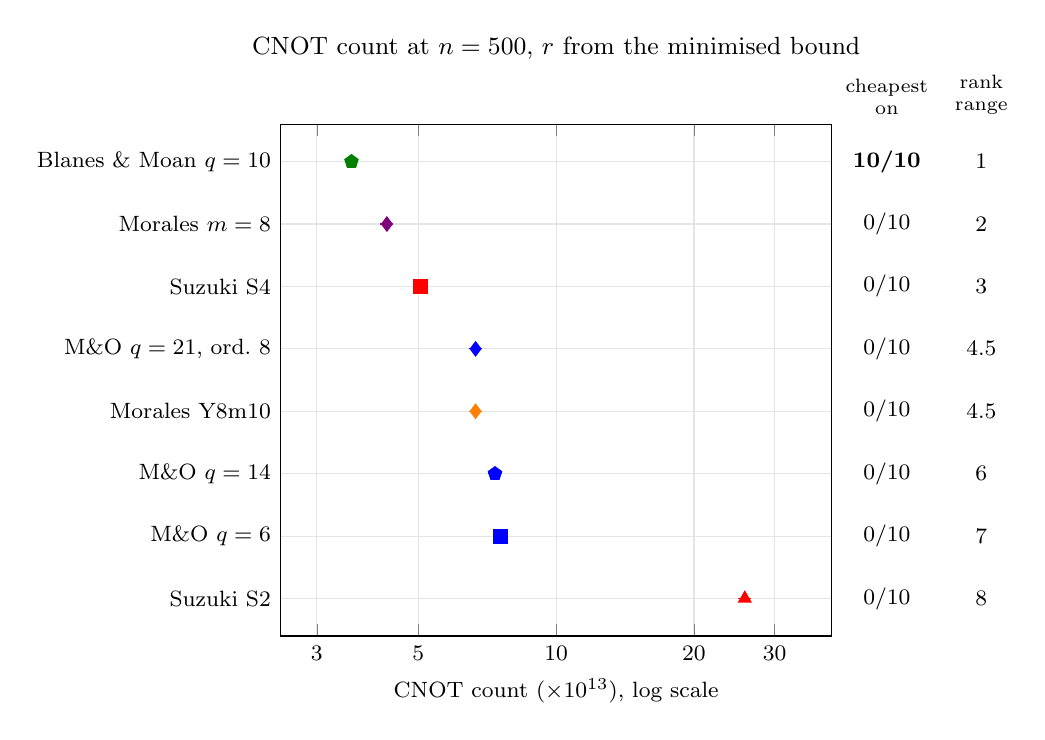
\begin{tikzpicture}
  \begin{semilogxaxis}[
    scale only axis, clip=false,
    at={(0cm,0cm)}, anchor=south west,
    width=7.0cm, height=6.5cm,
    title={CNOT count at $n = 500$, $r$ from the minimised bound}, title style={font=\small, yshift=14pt},
    xlabel={CNOT count ($\times 10^{13}$), log scale}, xlabel style={font=\footnotesize},
    xmin=2.5e+13, xmax=4e+14, xtick={3e+13,5e+13,1e+14,2e+14,3e+14}, xticklabels={3,5,10,20,30},
    xminorticks=false,
    y dir=reverse, ymin=0.4, ymax=8.6, ytick={1,2,3,4,5,6,7,8},
    yticklabels={{Blanes \& Moan $q=10$},{Morales $m=8$},{Suzuki S4},{M\&O $q=21$, ord.~8},{Morales Y8m10},{M\&O $q=14$},{M\&O $q=6$},{Suzuki S2}},
    tick label style={font=\footnotesize}, ytick style={draw=none},
    xmajorgrids=true, ymajorgrids=true, grid style={black!10},
  ]
    \addplot[green!50!black, only marks, mark=pentagon*, mark size=2.4pt, mark options={solid, fill=green!50!black, line width=0.6pt}, error bars/.cd, x dir=both, x explicit, error bar style={solid, line width=0.6pt}] coordinates {
      (3.57103e+13,1) += (0,0) -= (0,0)
    };
    \addplot[violet, only marks, mark=diamond*, mark size=2.4pt, mark options={solid, fill=violet, line width=0.6pt}, error bars/.cd, x dir=both, x explicit, error bar style={solid, line width=0.6pt}] coordinates {
      (4.26685e+13,2) += (0,0) -= (0,0)
    };
    \addplot[red, only marks, mark=square*, mark size=2.4pt, mark options={solid, fill=red, line width=0.6pt}, error bars/.cd, x dir=both, x explicit, error bar style={solid, line width=0.6pt}] coordinates {
      (5.05115e+13,3) += (0,0) -= (0,0)
    };
    \addplot[blue, only marks, mark=diamond*, mark size=2.4pt, mark options={solid, fill=blue, line width=0.6pt}, error bars/.cd, x dir=both, x explicit, error bar style={solid, line width=0.6pt}] coordinates {
      (6.66564e+13,4) += (0,0) -= (0,0)
    };
    \addplot[orange, only marks, mark=diamond*, mark size=2.4pt, mark options={solid, fill=orange, line width=0.6pt}, error bars/.cd, x dir=both, x explicit, error bar style={solid, line width=0.6pt}] coordinates {
      (6.66564e+13,5) += (0,0) -= (0,0)
    };
    \addplot[blue, only marks, mark=pentagon*, mark size=2.4pt, mark options={solid, fill=blue, line width=0.6pt}, error bars/.cd, x dir=both, x explicit, error bar style={solid, line width=0.6pt}] coordinates {
      (7.34983e+13,6) += (0,0) -= (0,0)
    };
    \addplot[blue, only marks, mark=square*, mark size=2.4pt, mark options={solid, fill=blue, line width=0.6pt}, error bars/.cd, x dir=both, x explicit, error bar style={solid, line width=0.6pt}] coordinates {
      (7.5521e+13,7) += (0,0) -= (0,0)
    };
    \addplot[red, only marks, mark=triangle*, mark size=2.4pt, mark options={solid, fill=red, line width=0.6pt}, error bars/.cd, x dir=both, x explicit, error bar style={solid, line width=0.6pt}] coordinates {
      (2.58204e+14,8) += (0,0) -= (0,0)
    };
    \node[anchor=south, font=\scriptsize, align=center] at ([xshift=0.7cm]axis cs:4e+14,0.4) {cheapest\\on};
    \node[anchor=south, font=\scriptsize, align=center] at ([xshift=1.9cm]axis cs:4e+14,0.4) {rank\\range};
    \node[font=\footnotesize\bfseries] at ([xshift=0.7cm]axis cs:4e+14,1) {10/10};
    \node[font=\footnotesize] at ([xshift=1.9cm]axis cs:4e+14,1) {1};
    \node[font=\footnotesize] at ([xshift=0.7cm]axis cs:4e+14,2) {0/10};
    \node[font=\footnotesize] at ([xshift=1.9cm]axis cs:4e+14,2) {2};
    \node[font=\footnotesize] at ([xshift=0.7cm]axis cs:4e+14,3) {0/10};
    \node[font=\footnotesize] at ([xshift=1.9cm]axis cs:4e+14,3) {3};
    \node[font=\footnotesize] at ([xshift=0.7cm]axis cs:4e+14,4) {0/10};
    \node[font=\footnotesize] at ([xshift=1.9cm]axis cs:4e+14,4) {4.5};
    \node[font=\footnotesize] at ([xshift=0.7cm]axis cs:4e+14,5) {0/10};
    \node[font=\footnotesize] at ([xshift=1.9cm]axis cs:4e+14,5) {4.5};
    \node[font=\footnotesize] at ([xshift=0.7cm]axis cs:4e+14,6) {0/10};
    \node[font=\footnotesize] at ([xshift=1.9cm]axis cs:4e+14,6) {6};
    \node[font=\footnotesize] at ([xshift=0.7cm]axis cs:4e+14,7) {0/10};
    \node[font=\footnotesize] at ([xshift=1.9cm]axis cs:4e+14,7) {7};
    \node[font=\footnotesize] at ([xshift=0.7cm]axis cs:4e+14,8) {0/10};
    \node[font=\footnotesize] at ([xshift=1.9cm]axis cs:4e+14,8) {8};
  \end{semilogxaxis}
\end{tikzpicture}
  \end{fitwidth}
  \caption{CNOT count against system size, $r$ from the minimised bound: full range and $n = 200$--$500$ enlarged (top); count at $n = 500$ over seeds (bottom). $r$ from the minimised norm bound (Childs et al.\ 2018 Def.~2, extended to every formula by counting $2q$ sweeps), computed at every $n$; no fit, no extrapolation. Same on all 10 seeds, so no spread; M\&O $q=21$ and Morales Y8m10 coincide (same order and $q$).}
\end{figure}
\clearpage
\pagelabel{3}{T count}{Measured $r$}{power-law fit on measured $n = 5$--$11$, extrapolated to $n = 500$}{As in the thesis (Figure~4.4)}
\begin{figure}[H]

  \centering
  \begin{fitwidth}
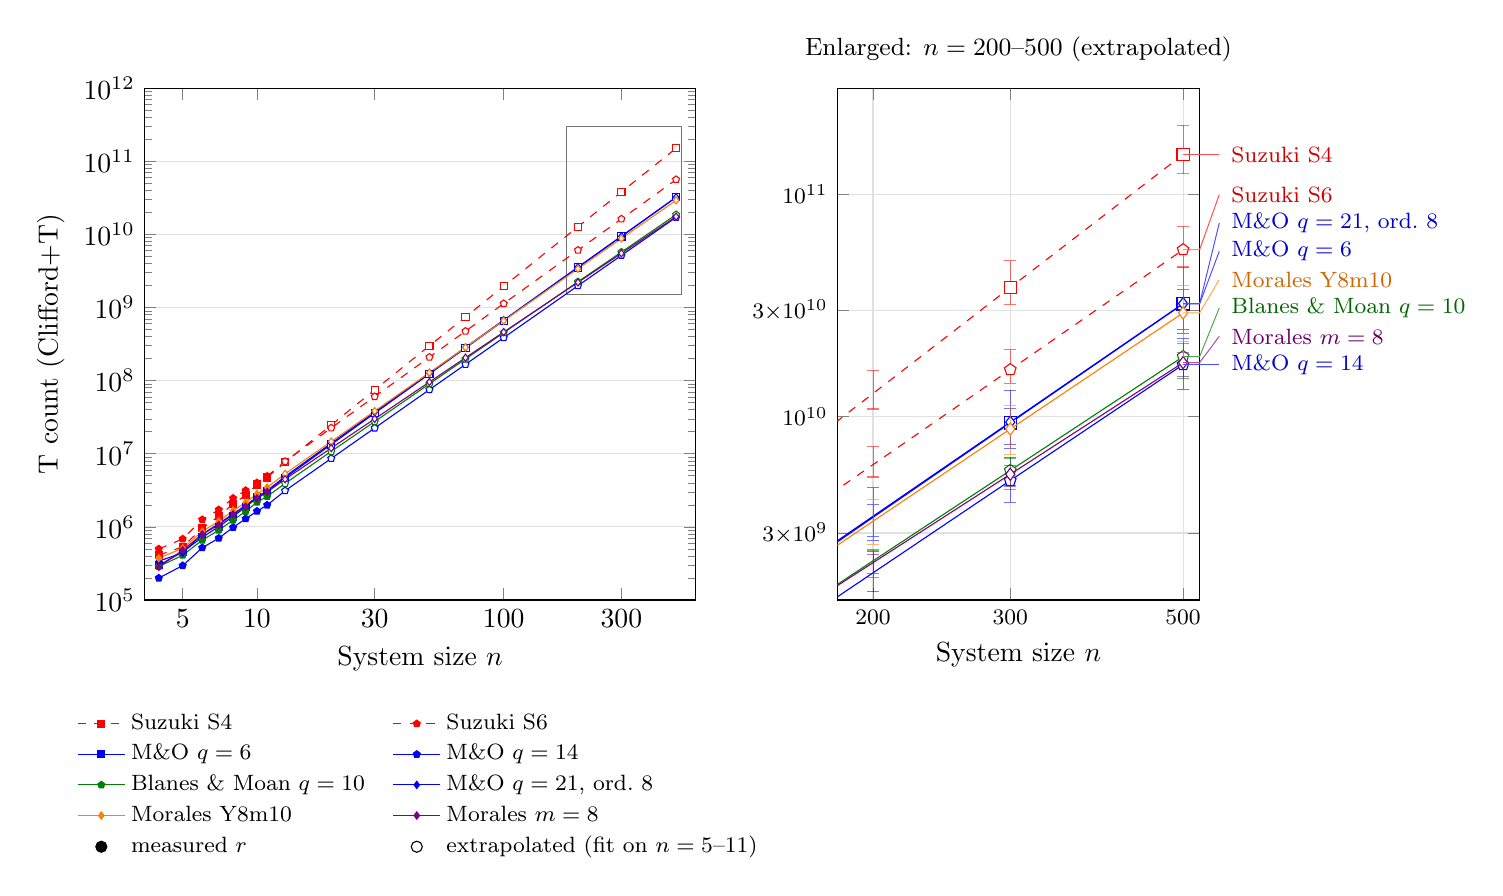
\begin{tikzpicture}
  \begin{loglogaxis}[
    name=main, scale only axis,
    width=7.0cm, height=6.5cm,
    xlabel={System size $n$},
    ylabel={T count (Clifford+T)},
    xtick={5,10,30,100,300}, xticklabels={5,10,30,100,300},
    xmin=3.5, xmax=600, ymin=100000, ymax=1e+12,
    ymajorgrids=true, grid style={black!12},
    legend style={at={(0.5,-0.2)}, anchor=north, draw=none, font=\footnotesize,
      legend columns=2, /tikz/every even column/.append style={column sep=8pt}},
    legend cell align=left,
  ]
    \draw[black!55, line width=0.5pt] (axis cs:180,1.5e+09) rectangle (axis cs:525,3e+11);
    \addplot[red, dashed, mark=square*, mark size=1.3pt, mark options={solid, fill=red}] coordinates {
      (4,410227)
      (5,535141)
      (6,956087)
      (7,1.39859e+06)
      (8,2.05215e+06)
      (9,2.71254e+06)
      (10,3.81418e+06)
      (11,4.74467e+06)
    };
    \addlegendentry{Suzuki S4}
    \addplot[red, dashed, mark=square*, mark size=1.3pt, mark options={solid, fill=white}, mark indices={2,...,10}, forget plot] coordinates {
      (11,4.74467e+06)
      (13,7.66257e+06)
      (20,2.47721e+07)
      (30,7.47488e+07)
      (50,2.99557e+08)
      (70,7.41804e+08)
      (100,1.95329e+09)
      (200,1.27159e+10)
      (300,3.81078e+10)
      (500,1.5088e+11)
    };
    \addplot[red, dashed, mark=pentagon*, mark size=1.3pt, mark options={solid, fill=red}] coordinates {
      (4,498655)
      (5,683636)
      (6,1.25709e+06)
      (7,1.71681e+06)
      (8,2.46342e+06)
      (9,3.14791e+06)
      (10,4.01292e+06)
      (11,4.938e+06)
    };
    \addlegendentry{Suzuki S6}
    \addplot[red, dashed, mark=pentagon*, mark size=1.3pt, mark options={solid, fill=white}, mark indices={2,...,10}, forget plot] coordinates {
      (11,4.938e+06)
      (13,7.85273e+06)
      (20,2.25571e+07)
      (30,6.05362e+07)
      (50,2.09429e+08)
      (70,4.74592e+08)
      (100,1.13273e+09)
      (200,6.08751e+09)
      (300,1.62764e+10)
      (500,5.631e+10)
    };
    \addplot[blue, solid, mark=square*, mark size=1.3pt, mark options={solid, fill=blue}] coordinates {
      (4,298204)
      (5,454337)
      (6,719342)
      (7,1.00507e+06)
      (8,1.38971e+06)
      (9,1.87541e+06)
      (10,2.57989e+06)
      (11,3.07213e+06)
    };
    \addlegendentry{M\&O $q=6$}
    \addplot[blue, solid, mark=square*, mark size=1.3pt, mark options={solid, fill=white}, mark indices={2,...,10}, forget plot] coordinates {
      (11,3.07213e+06)
      (13,4.68293e+06)
      (20,1.33975e+07)
      (30,3.58209e+07)
      (50,1.23593e+08)
      (70,2.79089e+08)
      (100,6.61509e+08)
      (200,3.52821e+09)
      (300,9.37974e+09)
      (500,3.21589e+10)
    };
    \addplot[blue, solid, mark=pentagon*, mark size=1.3pt, mark options={solid, fill=blue}] coordinates {
      (4,199644)
      (5,295456)
      (6,517803)
      (7,700110)
      (8,982626)
      (9,1.29212e+06)
      (10,1.63772e+06)
      (11,1.98699e+06)
    };
    \addlegendentry{M\&O $q=14$}
    \addplot[blue, solid, mark=pentagon*, mark size=1.3pt, mark options={solid, fill=white}, mark indices={2,...,10}, forget plot] coordinates {
      (11,1.98699e+06)
      (13,3.11874e+06)
      (20,8.61978e+06)
      (30,2.2459e+07)
      (50,7.52655e+07)
      (70,1.66795e+08)
      (100,3.86553e+08)
      (200,1.98691e+09)
      (300,5.16555e+09)
      (500,1.71426e+10)
    };
    \addplot[green!50!black, solid, mark=pentagon*, mark size=1.3pt, mark options={solid, fill=green!50!black}] coordinates {
      (4,287233)
      (5,408923)
      (6,658784)
      (7,901238)
      (8,1.23945e+06)
      (9,1.62436e+06)
      (10,2.1788e+06)
      (11,2.60871e+06)
    };
    \addlegendentry{Blanes \& Moan $q=10$}
    \addplot[green!50!black, solid, mark=pentagon*, mark size=1.3pt, mark options={solid, fill=white}, mark indices={2,...,10}, forget plot] coordinates {
      (11,2.60871e+06)
      (13,3.9301e+06)
      (20,1.0774e+07)
      (30,2.7548e+07)
      (50,9.03062e+07)
      (70,1.9751e+08)
      (100,4.51462e+08)
      (200,2.24975e+09)
      (300,5.73099e+09)
      (500,1.86331e+10)
    };
    \addplot[blue, solid, mark=diamond*, mark size=1.3pt, mark options={solid, fill=blue}] coordinates {
      (4,338991)
      (5,443831)
      (6,791120)
      (7,1.1119e+06)
      (8,1.50621e+06)
      (9,1.97285e+06)
      (10,2.54893e+06)
      (11,3.13956e+06)
    };
    \addlegendentry{M\&O $q=21$, ord.~8}
    \addplot[blue, solid, mark=diamond*, mark size=1.3pt, mark options={solid, fill=white}, mark indices={2,...,10}, forget plot] coordinates {
      (11,3.13956e+06)
      (13,4.88976e+06)
      (20,1.39079e+07)
      (30,3.70353e+07)
      (50,1.2702e+08)
      (70,2.85327e+08)
      (100,6.73578e+08)
      (200,3.56917e+09)
      (300,9.45042e+09)
      (500,3.22461e+10)
    };
    \addplot[orange, solid, mark=diamond*, mark size=1.3pt, mark options={solid, fill=orange}] coordinates {
      (4,373838)
      (5,509327)
      (6,864458)
      (7,1.19952e+06)
      (8,1.66587e+06)
      (9,2.15577e+06)
      (10,2.81799e+06)
      (11,3.46189e+06)
    };
    \addlegendentry{Morales Y8m10}
    \addplot[orange, solid, mark=diamond*, mark size=1.3pt, mark options={solid, fill=white}, mark indices={2,...,10}, forget plot] coordinates {
      (11,3.46189e+06)
      (13,5.32463e+06)
      (20,1.47085e+07)
      (30,3.84186e+07)
      (50,1.28596e+08)
      (70,2.84865e+08)
      (100,6.59306e+08)
      (200,3.39046e+09)
      (300,8.80299e+09)
      (500,2.92891e+10)
    };
    \addplot[violet, solid, mark=diamond*, mark size=1.3pt, mark options={solid, fill=violet}] coordinates {
      (4,283483)
      (5,480273)
      (6,790926)
      (7,1.06227e+06)
      (8,1.48074e+06)
      (9,1.89288e+06)
      (10,2.4461e+06)
      (11,3.00394e+06)
    };
    \addlegendentry{Morales $m=8$}
    \addplot[violet, solid, mark=diamond*, mark size=1.3pt, mark options={solid, fill=white}, mark indices={2,...,10}, forget plot] coordinates {
      (11,3.00394e+06)
      (13,4.48114e+06)
      (20,1.19454e+07)
      (30,3.00095e+07)
      (50,9.5688e+07)
      (70,2.05711e+08)
      (100,4.61972e+08)
      (200,2.2065e+09)
      (300,5.51227e+09)
      (500,1.75035e+10)
    };
    \addlegendimage{only marks, black, mark=*, mark options={solid, fill=black}}
    \addlegendentry{measured $r$}
    \addlegendimage{only marks, black, mark=*, mark options={solid, fill=white}}
    \addlegendentry{extrapolated (fit on $n = 5$--$11$)}
  \end{loglogaxis}
  \begin{loglogaxis}[
    scale only axis,
    at={(8.8cm,0cm)}, anchor=south west,
    width=4.6cm, height=6.5cm,
    title={Enlarged: $n = 200$--$500$ (extrapolated)}, title style={font=\small},
    xlabel={System size $n$},
    xtick={200,300,500}, xticklabels={200,300,500}, xminorticks=false,
    ytick={3e+09,1e+10,3e+10,1e+11}, yticklabels={{$3{\times}10^{9}$},{$10^{10}$},{$3{\times}10^{10}$},{$10^{11}$}}, yminorticks=false,
    xmin=180, xmax=525, ymin=1.5e+09, ymax=3e+11,
    xmajorgrids=true, ymajorgrids=true, grid style={black!12}, tick label style={font=\footnotesize},
    clip mode=individual,
  ]
    \addplot[red, dashed, mark=square*, mark size=2.2pt, mark options={solid, fill=white}, mark indices={2,...,10}, forget plot, error bars/.cd, y dir=both, y explicit, error bar style={solid, line width=0.35pt, opacity=0.55}] coordinates {
      (11,4.74467e+06)
      (13,7.66257e+06) += (0,387782) -= (0,206484)
      (20,2.47721e+07) += (0,2.00435e+06) -= (0,1.20859e+06)
      (30,7.47488e+07) += (0,8.81613e+06) -= (0,6.58761e+06)
      (50,2.99557e+08) += (0,4.65816e+07) -= (0,2.86018e+07)
      (70,7.41804e+08) += (0,1.31839e+08) -= (0,7.07925e+07)
      (100,1.95329e+09) += (0,4.06516e+08) -= (0,2.27538e+08)
      (200,1.27159e+10) += (0,3.44947e+09) -= (0,1.88592e+09)
      (300,3.81078e+10) += (0,1.21917e+10) -= (0,6.09671e+09)
      (500,1.5088e+11) += (0,5.3077e+10) -= (0,2.70956e+10)
    };
    \addplot[red, dashed, mark=pentagon*, mark size=2.2pt, mark options={solid, fill=white}, mark indices={2,...,10}, forget plot, error bars/.cd, y dir=both, y explicit, error bar style={solid, line width=0.35pt, opacity=0.55}] coordinates {
      (11,4.938e+06)
      (13,7.85273e+06) += (0,300450) -= (0,160976)
      (20,2.25571e+07) += (0,1.11956e+06) -= (0,1.00763e+06)
      (30,6.05362e+07) += (0,3.59495e+06) -= (0,2.84472e+06)
      (50,2.09429e+08) += (0,1.94953e+07) -= (0,1.38993e+07)
      (70,4.74592e+08) += (0,6.38993e+07) -= (0,3.83182e+07)
      (100,1.13273e+09) += (0,1.64668e+08) -= (0,1.01944e+08)
      (200,6.08751e+09) += (0,1.27029e+09) -= (0,7.27509e+08)
      (300,1.62764e+10) += (0,3.70913e+09) -= (0,2.14677e+09)
      (500,5.631e+10) += (0,1.54407e+10) -= (0,8.83844e+09)
    };
    \addplot[blue, solid, mark=square*, mark size=2.2pt, mark options={solid, fill=white}, mark indices={2,...,10}, forget plot, error bars/.cd, y dir=both, y explicit, error bar style={solid, line width=0.35pt, opacity=0.55}] coordinates {
      (11,3.07213e+06)
      (13,4.68293e+06) += (0,356548) -= (0,198754)
      (20,1.33975e+07) += (0,1.57555e+06) -= (0,835830)
      (30,3.58209e+07) += (0,5.86251e+06) -= (0,3.55025e+06)
      (50,1.23593e+08) += (0,2.50475e+07) -= (0,1.49872e+07)
      (70,2.79089e+08) += (0,7.04831e+07) -= (0,4.14157e+07)
      (100,6.61509e+08) += (0,1.94197e+08) -= (0,1.14688e+08)
      (200,3.52821e+09) += (0,1.26118e+09) -= (0,7.4489e+08)
      (300,9.37974e+09) += (0,3.79409e+09) -= (0,2.16652e+09)
      (500,3.21589e+10) += (0,1.48961e+10) -= (0,8.4356e+09)
    };
    \addplot[blue, solid, mark=pentagon*, mark size=2.2pt, mark options={solid, fill=white}, mark indices={2,...,10}, forget plot, error bars/.cd, y dir=both, y explicit, error bar style={solid, line width=0.35pt, opacity=0.55}] coordinates {
      (11,1.98699e+06)
      (13,3.11874e+06) += (0,57718.4) -= (0,105462)
      (20,8.61978e+06) += (0,566221) -= (0,428091)
      (30,2.2459e+07) += (0,2.19943e+06) -= (0,1.58811e+06)
      (50,7.52655e+07) += (0,9.82788e+06) -= (0,7.79298e+06)
      (70,1.66795e+08) += (0,2.71474e+07) -= (0,2.02453e+07)
      (100,3.86553e+08) += (0,7.14752e+07) -= (0,5.46946e+07)
      (200,1.98691e+09) += (0,4.88484e+08) -= (0,3.55086e+08)
      (300,5.16555e+09) += (0,1.40651e+09) -= (0,1.03303e+09)
      (500,1.71426e+10) += (0,5.38038e+09) -= (0,3.83706e+09)
    };
    \addplot[green!50!black, solid, mark=pentagon*, mark size=2.2pt, mark options={solid, fill=white}, mark indices={2,...,10}, forget plot, error bars/.cd, y dir=both, y explicit, error bar style={solid, line width=0.35pt, opacity=0.55}] coordinates {
      (11,2.60871e+06)
      (13,3.9301e+06) += (0,68836) -= (0,87804)
      (20,1.0774e+07) += (0,460669) -= (0,649855)
      (30,2.7548e+07) += (0,1.70443e+06) -= (0,1.9026e+06)
      (50,9.03062e+07) += (0,6.58258e+06) -= (0,8.73882e+06)
      (70,1.9751e+08) += (0,1.7158e+07) -= (0,2.14673e+07)
      (100,4.51462e+08) += (0,4.29653e+07) -= (0,5.62649e+07)
      (200,2.24975e+09) += (0,2.68432e+08) -= (0,3.56254e+08)
      (300,5.73099e+09) += (0,7.68518e+08) -= (0,1.04131e+09)
      (500,1.86331e+10) += (0,2.68049e+09) -= (0,3.81581e+09)
    };
    \addplot[blue, solid, mark=diamond*, mark size=2.2pt, mark options={solid, fill=white}, mark indices={2,...,10}, forget plot, error bars/.cd, y dir=both, y explicit, error bar style={solid, line width=0.35pt, opacity=0.55}] coordinates {
      (11,3.13956e+06)
      (13,4.88976e+06) += (0,56791) -= (0,186319)
      (20,1.39079e+07) += (0,486906) -= (0,907256)
      (30,3.70353e+07) += (0,1.60026e+06) -= (0,3.14339e+06)
      (50,1.2702e+08) += (0,8.2286e+06) -= (0,1.46677e+07)
      (70,2.85327e+08) += (0,2.31775e+07) -= (0,3.56762e+07)
      (100,6.73578e+08) += (0,6.27389e+07) -= (0,1.02361e+08)
      (200,3.56917e+09) += (0,4.59913e+08) -= (0,6.71365e+08)
      (300,9.45042e+09) += (0,1.40818e+09) -= (0,1.97079e+09)
      (500,3.22461e+10) += (0,5.17455e+09) -= (0,7.59363e+09)
    };
    \addplot[orange, solid, mark=diamond*, mark size=2.2pt, mark options={solid, fill=white}, mark indices={2,...,10}, forget plot, error bars/.cd, y dir=both, y explicit, error bar style={solid, line width=0.35pt, opacity=0.55}] coordinates {
      (11,3.46189e+06)
      (13,5.32463e+06) += (0,272075) -= (0,227581)
      (20,1.47085e+07) += (0,1.14689e+06) -= (0,1.13279e+06)
      (30,3.84186e+07) += (0,3.78324e+06) -= (0,3.5671e+06)
      (50,1.28596e+08) += (0,1.83792e+07) -= (0,1.61923e+07)
      (70,2.84865e+08) += (0,4.67169e+07) -= (0,4.26348e+07)
      (100,6.59306e+08) += (0,1.2942e+08) -= (0,1.13282e+08)
      (200,3.39046e+09) += (0,8.63829e+08) -= (0,7.1373e+08)
      (300,8.80299e+09) += (0,2.42332e+09) -= (0,2.02459e+09)
      (500,2.92891e+10) += (0,9.53382e+09) -= (0,7.5792e+09)
    };
    \addplot[violet, solid, mark=diamond*, mark size=2.2pt, mark options={solid, fill=white}, mark indices={2,...,10}, forget plot, error bars/.cd, y dir=both, y explicit, error bar style={solid, line width=0.35pt, opacity=0.55}] coordinates {
      (11,3.00394e+06)
      (13,4.48114e+06) += (0,71643.2) -= (0,105161)
      (20,1.19454e+07) += (0,365553) -= (0,348003)
      (30,3.00095e+07) += (0,1.1417e+06) -= (0,1.11385e+06)
      (50,9.5688e+07) += (0,5.37813e+06) -= (0,4.85e+06)
      (70,2.05711e+08) += (0,1.29501e+07) -= (0,1.22873e+07)
      (100,4.61972e+08) += (0,3.26388e+07) -= (0,3.73721e+07)
      (200,2.2065e+09) += (0,1.93245e+08) -= (0,2.24446e+08)
      (300,5.51227e+09) += (0,5.39536e+08) -= (0,6.30311e+08)
      (500,1.75035e+10) += (0,1.90596e+09) -= (0,2.33772e+09)
    };
    \draw[red!70, line width=0.35pt] (axis cs:500,1.5088e+11) -- (axis cs:525,1.5088e+11) -- ([xshift=0.25cm]axis cs:525,1.5088e+11);
    \node[anchor=west, font=\footnotesize, text=red!80!black] at ([xshift=0.28cm]axis cs:525,1.5088e+11) {Suzuki S4};
    \draw[red!70, line width=0.35pt] (axis cs:500,5.631e+10) -- (axis cs:525,5.631e+10) -- ([xshift=0.25cm]axis cs:525,9.97072e+10);
    \node[anchor=west, font=\footnotesize, text=red!80!black] at ([xshift=0.28cm]axis cs:525,9.97072e+10) {Suzuki S6};
    \draw[blue!70, line width=0.35pt] (axis cs:500,3.21589e+10) -- (axis cs:525,3.21589e+10) -- ([xshift=0.25cm]axis cs:525,5.54426e+10);
    \node[anchor=west, font=\footnotesize, text=blue!80!black] at ([xshift=0.28cm]axis cs:525,5.54426e+10) {M\&O $q=6$};
    \draw[blue!70, line width=0.35pt] (axis cs:500,1.71426e+10) -- (axis cs:525,1.71426e+10) -- ([xshift=0.25cm]axis cs:525,1.71426e+10);
    \node[anchor=west, font=\footnotesize, text=blue!80!black] at ([xshift=0.28cm]axis cs:525,1.71426e+10) {M\&O $q=14$};
    \draw[green!50!black!70, line width=0.35pt] (axis cs:500,1.86331e+10) -- (axis cs:525,1.86331e+10) -- ([xshift=0.25cm]axis cs:525,3.0829e+10);
    \node[anchor=west, font=\footnotesize, text=green!50!black!80!black] at ([xshift=0.28cm]axis cs:525,3.0829e+10) {Blanes \& Moan $q=10$};
    \draw[blue!70, line width=0.35pt] (axis cs:500,3.22461e+10) -- (axis cs:525,3.22461e+10) -- ([xshift=0.25cm]axis cs:525,7.43507e+10);
    \node[anchor=west, font=\footnotesize, text=blue!80!black] at ([xshift=0.28cm]axis cs:525,7.43507e+10) {M\&O $q=21$, ord.~8};
    \draw[orange!70, line width=0.35pt] (axis cs:500,2.92891e+10) -- (axis cs:525,2.92891e+10) -- ([xshift=0.25cm]axis cs:525,4.1343e+10);
    \node[anchor=west, font=\footnotesize, text=orange!80!black] at ([xshift=0.28cm]axis cs:525,4.1343e+10) {Morales Y8m10};
    \draw[violet!70, line width=0.35pt] (axis cs:500,1.75035e+10) -- (axis cs:525,1.75035e+10) -- ([xshift=0.25cm]axis cs:525,2.29889e+10);
    \node[anchor=west, font=\footnotesize, text=violet!80!black] at ([xshift=0.28cm]axis cs:525,2.29889e+10) {Morales $m=8$};
  \end{loglogaxis}
\end{tikzpicture}
  \end{fitwidth}\par\bigskip
  \begin{fitwidth}
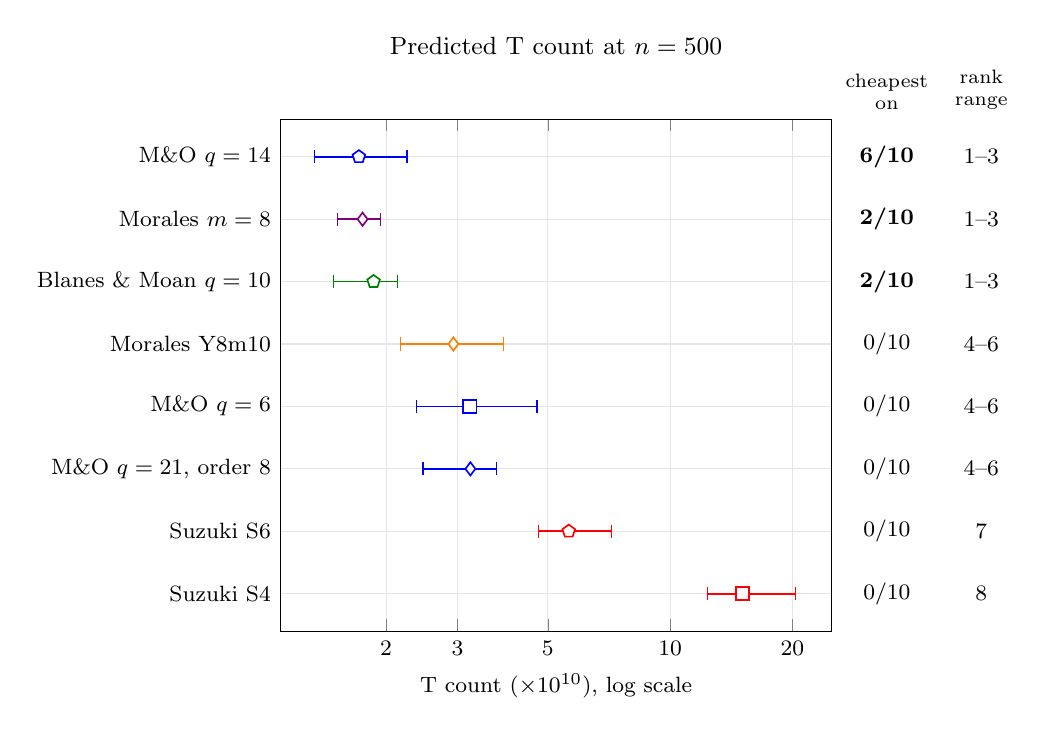
\begin{tikzpicture}
  \begin{semilogxaxis}[
    scale only axis, clip=false,
    at={(0cm,0cm)}, anchor=south west,
    width=7.0cm, height=6.5cm,
    title={Predicted T count at $n = 500$}, title style={font=\small, yshift=14pt},
    xlabel={T count ($\times 10^{10}$), log scale}, xlabel style={font=\footnotesize},
    xmin=1.1e+10, xmax=2.5e+11, xtick={2e+10,3e+10,5e+10,1e+11,2e+11}, xticklabels={2,3,5,10,20},
    xminorticks=false,
    y dir=reverse, ymin=0.4, ymax=8.6, ytick={1,2,3,4,5,6,7,8},
    yticklabels={{M\&O $q=14$},{Morales $m=8$},{Blanes \& Moan $q=10$},{Morales Y8m10},{M\&O $q=6$},{M\&O $q=21$, order 8},{Suzuki S6},{Suzuki S4}},
    tick label style={font=\footnotesize}, ytick style={draw=none},
    xmajorgrids=true, ymajorgrids=true, grid style={black!10},
  ]
    \addplot[blue, only marks, mark=pentagon*, mark size=2.4pt, mark options={solid, fill=white, line width=0.6pt}, error bars/.cd, x dir=both, x explicit, error bar style={solid, line width=0.6pt}] coordinates {
      (1.71426e+10,1) += (5.38038e+09,0) -= (3.83706e+09,0)
    };
    \addplot[violet, only marks, mark=diamond*, mark size=2.4pt, mark options={solid, fill=white, line width=0.6pt}, error bars/.cd, x dir=both, x explicit, error bar style={solid, line width=0.6pt}] coordinates {
      (1.75035e+10,2) += (1.90596e+09,0) -= (2.33772e+09,0)
    };
    \addplot[green!50!black, only marks, mark=pentagon*, mark size=2.4pt, mark options={solid, fill=white, line width=0.6pt}, error bars/.cd, x dir=both, x explicit, error bar style={solid, line width=0.6pt}] coordinates {
      (1.86331e+10,3) += (2.68049e+09,0) -= (3.81581e+09,0)
    };
    \addplot[orange, only marks, mark=diamond*, mark size=2.4pt, mark options={solid, fill=white, line width=0.6pt}, error bars/.cd, x dir=both, x explicit, error bar style={solid, line width=0.6pt}] coordinates {
      (2.92891e+10,4) += (9.53382e+09,0) -= (7.5792e+09,0)
    };
    \addplot[blue, only marks, mark=square*, mark size=2.4pt, mark options={solid, fill=white, line width=0.6pt}, error bars/.cd, x dir=both, x explicit, error bar style={solid, line width=0.6pt}] coordinates {
      (3.21589e+10,5) += (1.48961e+10,0) -= (8.4356e+09,0)
    };
    \addplot[blue, only marks, mark=diamond*, mark size=2.4pt, mark options={solid, fill=white, line width=0.6pt}, error bars/.cd, x dir=both, x explicit, error bar style={solid, line width=0.6pt}] coordinates {
      (3.22461e+10,6) += (5.17455e+09,0) -= (7.59363e+09,0)
    };
    \addplot[red, only marks, mark=pentagon*, mark size=2.4pt, mark options={solid, fill=white, line width=0.6pt}, error bars/.cd, x dir=both, x explicit, error bar style={solid, line width=0.6pt}] coordinates {
      (5.631e+10,7) += (1.54407e+10,0) -= (8.83844e+09,0)
    };
    \addplot[red, only marks, mark=square*, mark size=2.4pt, mark options={solid, fill=white, line width=0.6pt}, error bars/.cd, x dir=both, x explicit, error bar style={solid, line width=0.6pt}] coordinates {
      (1.5088e+11,8) += (5.3077e+10,0) -= (2.70956e+10,0)
    };
    \node[anchor=south, font=\scriptsize, align=center] at ([xshift=0.7cm]axis cs:2.5e+11,0.4) {cheapest\\on};
    \node[anchor=south, font=\scriptsize, align=center] at ([xshift=1.9cm]axis cs:2.5e+11,0.4) {rank\\range};
    \node[font=\footnotesize\bfseries] at ([xshift=0.7cm]axis cs:2.5e+11,1) {6/10};
    \node[font=\footnotesize] at ([xshift=1.9cm]axis cs:2.5e+11,1) {1--3};
    \node[font=\footnotesize\bfseries] at ([xshift=0.7cm]axis cs:2.5e+11,2) {2/10};
    \node[font=\footnotesize] at ([xshift=1.9cm]axis cs:2.5e+11,2) {1--3};
    \node[font=\footnotesize\bfseries] at ([xshift=0.7cm]axis cs:2.5e+11,3) {2/10};
    \node[font=\footnotesize] at ([xshift=1.9cm]axis cs:2.5e+11,3) {1--3};
    \node[font=\footnotesize] at ([xshift=0.7cm]axis cs:2.5e+11,4) {0/10};
    \node[font=\footnotesize] at ([xshift=1.9cm]axis cs:2.5e+11,4) {4--6};
    \node[font=\footnotesize] at ([xshift=0.7cm]axis cs:2.5e+11,5) {0/10};
    \node[font=\footnotesize] at ([xshift=1.9cm]axis cs:2.5e+11,5) {4--6};
    \node[font=\footnotesize] at ([xshift=0.7cm]axis cs:2.5e+11,6) {0/10};
    \node[font=\footnotesize] at ([xshift=1.9cm]axis cs:2.5e+11,6) {4--6};
    \node[font=\footnotesize] at ([xshift=0.7cm]axis cs:2.5e+11,7) {0/10};
    \node[font=\footnotesize] at ([xshift=1.9cm]axis cs:2.5e+11,7) {7};
    \node[font=\footnotesize] at ([xshift=0.7cm]axis cs:2.5e+11,8) {0/10};
    \node[font=\footnotesize] at ([xshift=1.9cm]axis cs:2.5e+11,8) {8};
  \end{semilogxaxis}
\end{tikzpicture}
  \end{fitwidth}
    \caption{T count against system size, extrapolated to $n = 500$: full range and $n = 200$--$500$ enlarged (top); predicted count at $n = 500$ over seeds (bottom)}
\end{figure}
\clearpage
\pagelabel{4}{T count}{Minimised bound $r$}{norm bound evaluated at every $n = 4$--$500$}{New; counterpart of Figure~4.4}
\begin{figure}[H]
  \centering
  \begin{fitwidth}
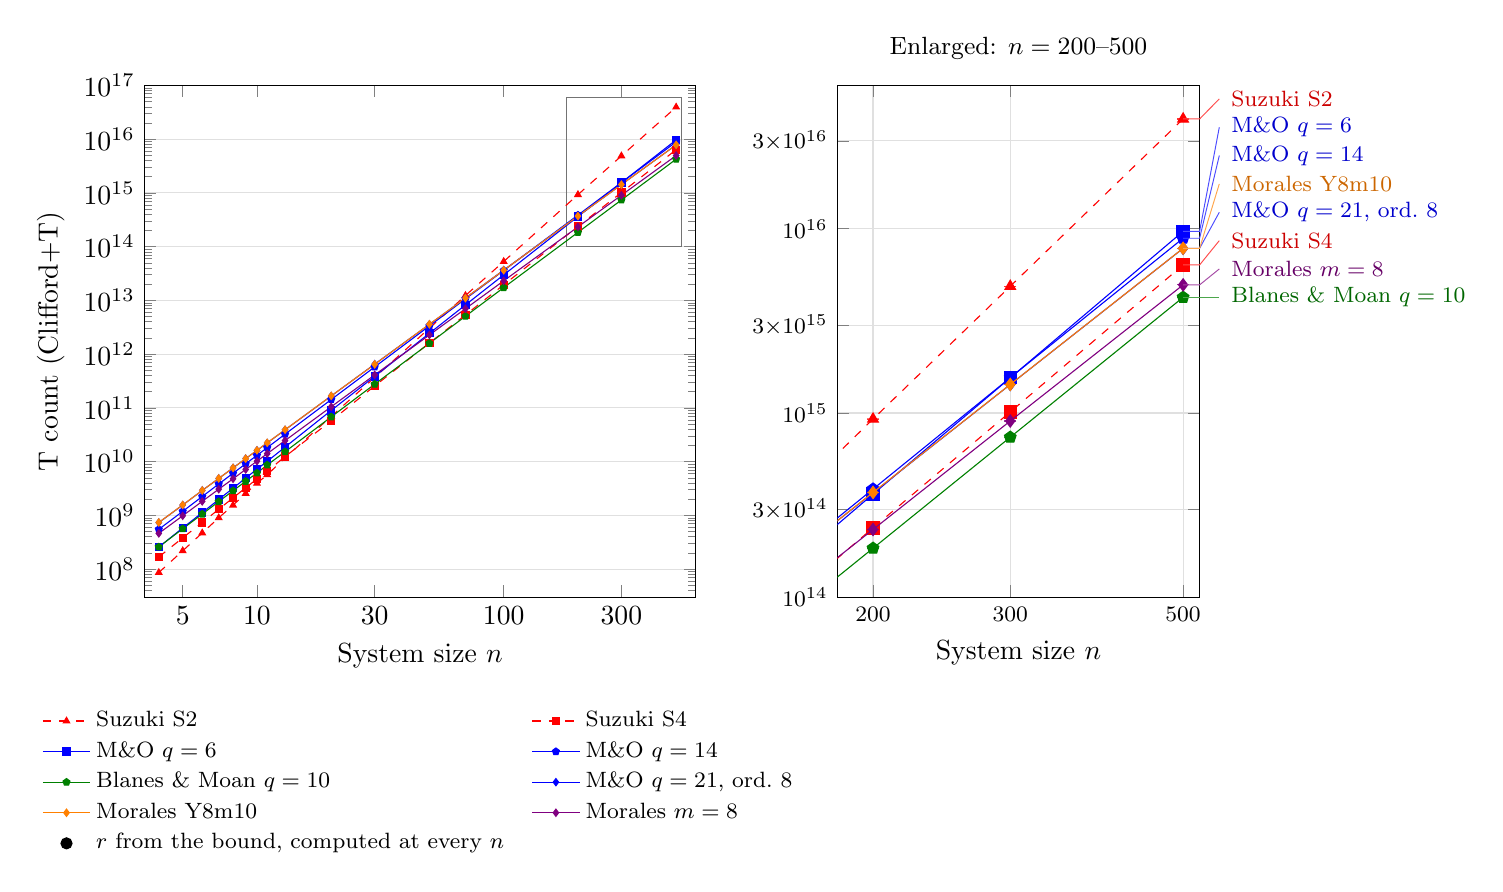
\begin{tikzpicture}
  \begin{loglogaxis}[
    name=main, scale only axis,
    width=7.0cm, height=6.5cm,
    xlabel={System size $n$},
    ylabel={T count (Clifford+T)},
    xtick={5,10,30,100,300}, xticklabels={5,10,30,100,300},
    xmin=3.5, xmax=600, ymin=3e+07, ymax=1e+17,
    ymajorgrids=true, grid style={black!12},
    legend style={at={(0.5,-0.2)}, anchor=north, draw=none, font=\footnotesize,
      legend columns=2, /tikz/every even column/.append style={column sep=8pt}},
    legend cell align=left,
  ]
    \draw[black!55, line width=0.5pt] (axis cs:180,1e+14) rectangle (axis cs:525,6e+16);
    \addplot[red, dashed, mark=triangle*, mark size=1.3pt, mark options={solid, fill=red}] coordinates {
      (4,8.62687e+07)
      (5,2.19039e+08)
      (6,4.70263e+08)
      (7,9.00087e+08)
      (8,1.54747e+09)
      (9,2.55535e+09)
      (10,3.94935e+09)
      (11,5.6951e+09)
      (13,1.17213e+10)
      (20,6.95434e+10)
      (30,3.68634e+11)
      (50,3.03699e+12)
      (70,1.2311e+13)
      (100,5.28099e+13)
      (200,9.27206e+14)
      (300,4.86931e+15)
      (500,3.9433e+16)
    };
    \addlegendentry{Suzuki S2}
    \addplot[red, dashed, mark=square*, mark size=1.3pt, mark options={solid, fill=red}] coordinates {
      (4,1.68074e+08)
      (5,3.82183e+08)
      (6,7.34359e+08)
      (7,1.30059e+09)
      (8,2.1159e+09)
      (9,3.26505e+09)
      (10,4.75134e+09)
      (11,6.64172e+09)
      (13,1.23961e+10)
      (20,5.76672e+10)
      (30,2.55507e+11)
      (50,1.6134e+12)
      (70,5.36739e+12)
      (100,1.94635e+13)
      (200,2.37836e+14)
      (300,1.01276e+15)
      (500,6.36193e+15)
    };
    \addlegendentry{Suzuki S4}
    \addplot[blue, solid, mark=square*, mark size=1.3pt, mark options={solid, fill=blue}] coordinates {
      (4,2.57703e+08)
      (5,5.81845e+08)
      (6,1.1242e+09)
      (7,1.97549e+09)
      (8,3.20668e+09)
      (9,4.94547e+09)
      (10,7.24806e+09)
      (11,1.0121e+10)
      (13,1.8635e+10)
      (20,8.96775e+10)
      (30,3.86026e+11)
      (50,2.43634e+12)
      (70,8.23766e+12)
      (100,2.97927e+13)
      (200,3.62747e+14)
      (300,1.55103e+15)
      (500,9.67956e+15)
    };
    \addlegendentry{M\&O $q=6$}
    \addplot[blue, solid, mark=pentagon*, mark size=1.3pt, mark options={solid, fill=blue}] coordinates {
      (4,5.50279e+08)
      (5,1.18765e+09)
      (6,2.24106e+09)
      (7,3.83354e+09)
      (8,6.07395e+09)
      (9,9.12076e+09)
      (10,1.30737e+10)
      (11,1.81679e+10)
      (13,3.24672e+10)
      (20,1.42981e+11)
      (30,5.77661e+11)
      (50,3.35535e+12)
      (70,1.06752e+13)
      (100,3.5985e+13)
      (200,3.86224e+14)
      (300,1.55395e+15)
      (500,8.87764e+15)
    };
    \addlegendentry{M\&O $q=14$}
    \addplot[green!50!black, solid, mark=pentagon*, mark size=1.3pt, mark options={solid, fill=green!50!black}] coordinates {
      (4,2.57673e+08)
      (5,5.6315e+08)
      (6,1.05686e+09)
      (7,1.80445e+09)
      (8,2.87407e+09)
      (9,4.3031e+09)
      (10,6.1567e+09)
      (11,8.65086e+09)
      (13,1.52563e+10)
      (20,6.80439e+10)
      (30,2.75827e+11)
      (50,1.59131e+12)
      (70,5.06469e+12)
      (100,1.72869e+13)
      (200,1.8438e+14)
      (300,7.38404e+14)
      (500,4.24434e+15)
    };
    \addlegendentry{Blanes \& Moan $q=10$}
    \addplot[blue, solid, mark=diamond*, mark size=1.3pt, mark options={solid, fill=blue}] coordinates {
      (4,7.34481e+08)
      (5,1.55769e+09)
      (6,2.90479e+09)
      (7,4.86765e+09)
      (8,7.64197e+09)
      (9,1.13807e+10)
      (10,1.61814e+10)
      (11,2.22474e+10)
      (13,3.90543e+10)
      (20,1.66264e+11)
      (30,6.50208e+11)
      (50,3.58857e+12)
      (70,1.10564e+13)
      (100,3.6558e+13)
      (200,3.69357e+14)
      (300,1.42755e+15)
      (500,7.82549e+15)
    };
    \addlegendentry{M\&O $q=21$, ord.~8}
    \addplot[orange, solid, mark=diamond*, mark size=1.3pt, mark options={solid, fill=orange}] coordinates {
      (4,7.38042e+08)
      (5,1.56206e+09)
      (6,2.90695e+09)
      (7,4.87222e+09)
      (8,7.64216e+09)
      (9,1.13482e+10)
      (10,1.62306e+10)
      (11,2.23956e+10)
      (13,3.91753e+10)
      (20,1.67039e+11)
      (30,6.45747e+11)
      (50,3.60051e+12)
      (70,1.10209e+13)
      (100,3.64014e+13)
      (200,3.70358e+14)
      (300,1.42803e+15)
      (500,7.83221e+15)
    };
    \addlegendentry{Morales Y8m10}
    \addplot[violet, solid, mark=diamond*, mark size=1.3pt, mark options={solid, fill=violet}] coordinates {
      (4,4.62885e+08)
      (5,9.82312e+08)
      (6,1.82446e+09)
      (7,3.07124e+09)
      (8,4.78934e+09)
      (9,7.15423e+09)
      (10,1.01945e+10)
      (11,1.40551e+10)
      (13,2.46574e+10)
      (20,1.04923e+11)
      (30,4.10346e+11)
      (50,2.27443e+12)
      (70,6.9995e+12)
      (100,2.31127e+13)
      (200,2.33015e+14)
      (300,9.04384e+14)
      (500,4.9572e+15)
    };
    \addlegendentry{Morales $m=8$}
    \addlegendimage{only marks, black, mark=*, mark options={solid, fill=black}}
    \addlegendentry{$r$ from the bound, computed at every $n$}
  \end{loglogaxis}
  \begin{loglogaxis}[
    scale only axis,
    at={(8.8cm,0cm)}, anchor=south west,
    width=4.6cm, height=6.5cm,
    title={Enlarged: $n = 200$--$500$}, title style={font=\small},
    xlabel={System size $n$},
    xtick={200,300,500}, xticklabels={200,300,500}, xminorticks=false,
    ytick={1e+14,3e+14,1e+15,3e+15,1e+16,3e+16}, yticklabels={{$10^{14}$},{$3{\times}10^{14}$},{$10^{15}$},{$3{\times}10^{15}$},{$10^{16}$},{$3{\times}10^{16}$}}, yminorticks=false,
    xmin=180, xmax=525, ymin=1e+14, ymax=6e+16,
    xmajorgrids=true, ymajorgrids=true, grid style={black!12}, tick label style={font=\footnotesize},
    clip mode=individual,
  ]
    \addplot[red, dashed, mark=triangle*, mark size=2.2pt, mark options={solid, fill=red}, forget plot, error bars/.cd, y dir=both, y explicit, error bar style={solid, line width=0.35pt, opacity=0.55}] coordinates {
      (4,8.62687e+07) += (0,254701) -= (0,194771)
      (5,2.19039e+08) += (0,643544) -= (0,819056)
      (6,4.70263e+08) += (0,1.23813e+06) -= (0,530628)
      (7,9.00087e+08) += (0,962832) -= (0,1.44425e+06)
      (8,1.54747e+09) += (0,2.15558e+06) -= (0,3.23337e+06)
      (9,2.55535e+09) += (0,2.89838e+06) -= (0,3.06888e+06)
      (10,3.94935e+09) += (0,5.14481e+06) -= (0,5.37867e+06)
      (11,5.6951e+09) += (0,9.95973e+06) -= (0,8.71476e+06)
      (13,1.17213e+10) += (0,1.66952e+07) -= (0,2.44007e+07)
      (20,6.95434e+10) += (0,6.5457e+07) -= (0,9.351e+07)
      (30,3.68634e+11) += (0,3.18716e+08) -= (0,3.12405e+08)
      (50,3.03699e+12) += (0,1.60687e+09) -= (0,2.19119e+09)
      (70,1.2311e+13) += (0,3.60743e+09) -= (0,6.01239e+09)
      (100,5.28099e+13) += (0,1.22698e+10) -= (0,2.62925e+10)
      (200,9.27206e+14) += (0,1.92571e+11) -= (0,2.84183e+11)
      (300,4.86931e+15) += (0,6.08906e+11) -= (0,5.89976e+11)
      (500,3.9433e+16) += (0,5.33124e+12) -= (0,4.16275e+12)
    };
    \addplot[red, dashed, mark=square*, mark size=2.2pt, mark options={solid, fill=red}, forget plot, error bars/.cd, y dir=both, y explicit, error bar style={solid, line width=0.35pt, opacity=0.55}] coordinates {
      (4,1.68074e+08) += (0,498813) -= (0,855581)
      (5,3.82183e+08) += (0,599539) -= (0,1.1299e+06)
      (6,7.34359e+08) += (0,1.0359e+06) -= (0,1.32667e+06)
      (7,1.30059e+09) += (0,3.15088e+06) -= (0,2.32311e+06)
      (8,2.1159e+09) += (0,4.77015e+06) -= (0,3.24221e+06)
      (9,3.26505e+09) += (0,3.92557e+06) -= (0,4.82569e+06)
      (10,4.75134e+09) += (0,9.75834e+06) -= (0,4.55389e+06)
      (11,6.64172e+09) += (0,1.06471e+07) -= (0,9.98681e+06)
      (13,1.23961e+10) += (0,2.66806e+07) -= (0,1.65344e+07)
      (20,5.76672e+10) += (0,5.43677e+07) -= (0,5.03268e+07)
      (30,2.55507e+11) += (0,1.57287e+08) -= (0,2.37194e+08)
      (50,1.6134e+12) += (0,7.97367e+08) -= (0,8.69855e+08)
      (70,5.36739e+12) += (0,1.4241e+09) -= (0,3.95303e+09)
      (100,1.94635e+13) += (0,3.95383e+09) -= (0,6.59654e+09)
      (200,2.37836e+14) += (0,4.63863e+10) -= (0,4.04794e+10)
      (300,1.01276e+15) += (0,2.51119e+11) -= (0,1.74858e+11)
      (500,6.36193e+15) += (0,8.36818e+11) -= (0,7.81907e+11)
    };
    \addplot[blue, solid, mark=square*, mark size=2.2pt, mark options={solid, fill=blue}, forget plot, error bars/.cd, y dir=both, y explicit, error bar style={solid, line width=0.35pt, opacity=0.55}] coordinates {
      (4,2.57703e+08) += (0,489346) -= (0,422994)
      (5,5.81845e+08) += (0,1.36067e+06) -= (0,1.24487e+06)
      (6,1.1242e+09) += (0,1.82538e+06) -= (0,2.28172e+06)
      (7,1.97549e+09) += (0,2.54798e+06) -= (0,3.4867e+06)
      (8,3.20668e+09) += (0,4.63237e+06) -= (0,4.25804e+06)
      (9,4.94547e+09) += (0,4.20688e+06) -= (0,3.95572e+06)
      (10,7.24806e+09) += (0,6.37141e+06) -= (0,3.43076e+06)
      (11,1.0121e+10) += (0,2.27997e+07) -= (0,1.86543e+07)
      (13,1.8635e+10) += (0,7.09356e+07) -= (0,2.50083e+07)
      (20,8.96775e+10) += (0,7.05769e+07) -= (0,7.24221e+07)
      (30,3.86026e+11) += (0,2.38796e+08) -= (0,2.81982e+08)
      (50,2.43634e+12) += (0,5.55288e+08) -= (0,6.73629e+08)
      (70,8.23766e+12) += (0,1.66709e+09) -= (0,2.97544e+09)
      (100,2.97927e+13) += (0,8.87602e+09) -= (0,6.56053e+09)
      (200,3.62747e+14) += (0,6.51651e+10) -= (0,3.95645e+10)
      (300,1.55103e+15) += (0,2.717e+11) -= (0,3.17384e+11)
      (500,9.67956e+15) += (0,5.50269e+11) -= (0,6.70955e+11)
    };
    \addplot[blue, solid, mark=pentagon*, mark size=2.2pt, mark options={solid, fill=blue}, forget plot, error bars/.cd, y dir=both, y explicit, error bar style={solid, line width=0.35pt, opacity=0.55}] coordinates {
      (4,5.50279e+08) += (0,622699) -= (0,1.02783e+06)
      (5,1.18765e+09) += (0,1.337e+06) -= (0,1.94243e+06)
      (6,2.24106e+09) += (0,1.71631e+06) -= (0,1.94772e+06)
      (7,3.83354e+09) += (0,4.14198e+06) -= (0,4.41811e+06)
      (8,6.07395e+09) += (0,4.86155e+06) -= (0,3.0526e+06)
      (9,9.12076e+09) += (0,5.94994e+06) -= (0,5.94994e+06)
      (10,1.30737e+10) += (0,1.51466e+07) -= (0,9.56959e+06)
      (11,1.81679e+10) += (0,2.40555e+07) -= (0,1.55095e+07)
      (13,3.24672e+10) += (0,6.13084e+07) -= (0,2.86106e+07)
      (20,1.42981e+11) += (0,1.20757e+08) -= (0,6.72289e+07)
      (30,5.77661e+11) += (0,1.54099e+08) -= (0,2.06559e+08)
      (50,3.35535e+12) += (0,8.38487e+08) -= (0,6.17407e+08)
      (70,1.06752e+13) += (0,2.26838e+09) -= (0,1.6304e+09)
      (100,3.5985e+13) += (0,5.10165e+09) -= (0,6.83838e+09)
      (200,3.86224e+14) += (0,3.68149e+10) -= (0,6.29063e+10)
      (300,1.55395e+15) += (0,1.27823e+11) -= (0,1.41186e+11)
      (500,8.87764e+15) += (0,5.80449e+11) -= (0,8.95269e+11)
    };
    \addplot[green!50!black, solid, mark=pentagon*, mark size=2.2pt, mark options={solid, fill=green!50!black}, forget plot, error bars/.cd, y dir=both, y explicit, error bar style={solid, line width=0.35pt, opacity=0.55}] coordinates {
      (4,2.57673e+08) += (0,248489) -= (0,309343)
      (5,5.6315e+08) += (0,775830) -= (0,1.01455e+06)
      (6,1.05686e+09) += (0,1.10789e+06) -= (0,977550)
      (7,1.80445e+09) += (0,1.69828e+06) -= (0,2.0342e+06)
      (8,2.87407e+09) += (0,2.41957e+06) -= (0,2.67427e+06)
      (9,4.3031e+09) += (0,3.01572e+06) -= (0,4.69112e+06)
      (10,6.1567e+09) += (0,3.25493e+06) -= (0,5.31067e+06)
      (11,8.65086e+09) += (0,1.35289e+07) -= (0,6.7912e+06)
      (13,1.52563e+10) += (0,3.49582e+07) -= (0,1.55457e+07)
      (20,6.80439e+10) += (0,3.72452e+07) -= (0,3.16476e+07)
      (30,2.75827e+11) += (0,7.1442e+07) -= (0,7.25496e+07)
      (50,1.59131e+12) += (0,5.35517e+08) -= (0,2.84152e+08)
      (70,5.06469e+12) += (0,9.45811e+08) -= (0,1.84772e+09)
      (100,1.72869e+13) += (0,1.78736e+09) -= (0,2.06234e+09)
      (200,1.8438e+14) += (0,1.4026e+10) -= (0,2.7037e+10)
      (300,7.38404e+14) += (0,1.15202e+11) -= (0,1.05701e+11)
      (500,4.24434e+15) += (0,3.04117e+11) -= (0,4.77675e+11)
    };
    \addplot[blue, solid, mark=diamond*, mark size=2.2pt, mark options={solid, fill=blue}, forget plot, error bars/.cd, y dir=both, y explicit, error bar style={solid, line width=0.35pt, opacity=0.55}] coordinates {
      (4,7.34481e+08) += (0,511034) -= (0,749958)
      (5,1.55769e+09) += (0,1.38558e+06) -= (0,1.07889e+06)
      (6,2.90479e+09) += (0,1.69888e+06) -= (0,1.51745e+06)
      (7,4.86765e+09) += (0,2.44822e+06) -= (0,1.86531e+06)
      (8,7.64197e+09) += (0,3.8236e+06) -= (0,6.5615e+06)
      (9,1.13807e+10) += (0,4.14092e+06) -= (0,3.03394e+06)
      (10,1.61814e+10) += (0,6.51912e+06) -= (0,6.20745e+06)
      (11,2.22474e+10) += (0,1.95609e+07) -= (0,1.48637e+07)
      (13,3.90543e+10) += (0,8.49347e+07) -= (0,1.90097e+07)
      (20,1.66264e+11) += (0,6.59301e+07) -= (0,5.36067e+07)
      (30,6.50208e+11) += (0,2.73974e+08) -= (0,2.71522e+08)
      (50,3.58857e+12) += (0,6.75107e+08) -= (0,3.87293e+08)
      (70,1.10564e+13) += (0,1.05747e+09) -= (0,1.86395e+09)
      (100,3.6558e+13) += (0,1.02735e+10) -= (0,6.09987e+09)
      (200,3.69357e+14) += (0,3.10001e+10) -= (0,4.56832e+10)
      (300,1.42755e+15) += (0,8.49399e+10) -= (0,1.02611e+11)
      (500,7.82549e+15) += (0,7.44269e+11) -= (0,6.18116e+11)
    };
    \addplot[orange, solid, mark=diamond*, mark size=2.2pt, mark options={solid, fill=orange}, forget plot, error bars/.cd, y dir=both, y explicit, error bar style={solid, line width=0.35pt, opacity=0.55}] coordinates {
      (4,7.38042e+08) += (0,633814) -= (0,793098)
      (5,1.56206e+09) += (0,958405) -= (0,1.4513e+06)
      (6,2.90695e+09) += (0,1.1051e+06) -= (0,1.78135e+06)
      (7,4.87222e+09) += (0,3.59073e+06) -= (0,5.73583e+06)
      (8,7.64216e+09) += (0,5.20828e+06) -= (0,5.01946e+06)
      (9,1.13482e+10) += (0,7.37986e+06) -= (0,2.66495e+06)
      (10,1.62306e+10) += (0,8.25929e+06) -= (0,8.36318e+06)
      (11,2.23956e+10) += (0,2.09765e+07) -= (0,1.44133e+07)
      (13,3.91753e+10) += (0,3.14174e+07) -= (0,2.05548e+07)
      (20,1.67039e+11) += (0,1.55028e+08) -= (0,8.40455e+07)
      (30,6.45747e+11) += (0,2.61102e+08) -= (0,1.9552e+08)
      (50,3.60051e+12) += (0,5.63072e+08) -= (0,8.56681e+08)
      (70,1.10209e+13) += (0,1.96888e+09) -= (0,8.29109e+08)
      (100,3.64014e+13) += (0,5.22387e+09) -= (0,3.99472e+09)
      (200,3.70358e+14) += (0,2.28961e+10) -= (0,2.80809e+10)
      (300,1.42803e+15) += (0,6.87325e+10) -= (0,1.23155e+11)
      (500,7.83221e+15) += (0,4.54015e+11) -= (0,4.74185e+11)
    };
    \addplot[violet, solid, mark=diamond*, mark size=2.2pt, mark options={solid, fill=violet}, forget plot, error bars/.cd, y dir=both, y explicit, error bar style={solid, line width=0.35pt, opacity=0.55}] coordinates {
      (4,4.62885e+08) += (0,780104) -= (0,528796)
      (5,9.82312e+08) += (0,1.48176e+06) -= (0,937440)
      (6,1.82446e+09) += (0,1.60683e+06) -= (0,1.64587e+06)
      (7,3.07124e+09) += (0,2.36332e+06) -= (0,2.23458e+06)
      (8,4.78934e+09) += (0,2.20923e+06) -= (0,2.63122e+06)
      (9,7.15423e+09) += (0,4.76997e+06) -= (0,4.93167e+06)
      (10,1.01945e+10) += (0,4.17918e+06) -= (0,1.11855e+07)
      (11,1.40551e+10) += (0,1.44391e+07) -= (0,1.01759e+07)
      (13,2.46574e+10) += (0,4.37623e+07) -= (0,2.12349e+07)
      (20,1.04923e+11) += (0,9.61261e+07) -= (0,5.06387e+07)
      (30,4.10346e+11) += (0,1.86107e+08) -= (0,1.11181e+08)
      (50,2.27443e+12) += (0,3.52663e+08) -= (0,3.25242e+08)
      (70,6.9995e+12) += (0,1.86748e+09) -= (0,1.06922e+09)
      (100,2.31127e+13) += (0,2.07608e+09) -= (0,2.58968e+09)
      (200,2.33015e+14) += (0,2.9222e+10) -= (0,3.29671e+10)
      (300,9.04384e+14) += (0,3.83419e+10) -= (0,7.27941e+10)
      (500,4.9572e+15) += (0,2.92503e+11) -= (0,2.97895e+11)
    };
    \draw[red!70, line width=0.35pt] (axis cs:500,3.9433e+16) -- (axis cs:525,3.9433e+16) -- ([xshift=0.25cm]axis cs:525,5.06848e+16);
    \node[anchor=west, font=\footnotesize, text=red!80!black] at ([xshift=0.28cm]axis cs:525,5.06848e+16) {Suzuki S2};
    \draw[red!70, line width=0.35pt] (axis cs:500,6.36193e+15) -- (axis cs:525,6.36193e+15) -- ([xshift=0.25cm]axis cs:525,8.62073e+15);
    \node[anchor=west, font=\footnotesize, text=red!80!black] at ([xshift=0.28cm]axis cs:525,8.62073e+15) {Suzuki S4};
    \draw[blue!70, line width=0.35pt] (axis cs:500,9.67956e+15) -- (axis cs:525,9.67956e+15) -- ([xshift=0.25cm]axis cs:525,3.5564e+16);
    \node[anchor=west, font=\footnotesize, text=blue!80!black] at ([xshift=0.28cm]axis cs:525,3.5564e+16) {M\&O $q=6$};
    \draw[blue!70, line width=0.35pt] (axis cs:500,8.87764e+15) -- (axis cs:525,8.87764e+15) -- ([xshift=0.25cm]axis cs:525,2.49542e+16);
    \node[anchor=west, font=\footnotesize, text=blue!80!black] at ([xshift=0.28cm]axis cs:525,2.49542e+16) {M\&O $q=14$};
    \draw[green!50!black!70, line width=0.35pt] (axis cs:500,4.24434e+15) -- (axis cs:525,4.24434e+15) -- ([xshift=0.25cm]axis cs:525,4.24434e+15);
    \node[anchor=west, font=\footnotesize, text=green!50!black!80!black] at ([xshift=0.28cm]axis cs:525,4.24434e+15) {Blanes \& Moan $q=10$};
    \draw[blue!70, line width=0.35pt] (axis cs:500,7.82549e+15) -- (axis cs:525,7.82549e+15) -- ([xshift=0.25cm]axis cs:525,1.2286e+16);
    \node[anchor=west, font=\footnotesize, text=blue!80!black] at ([xshift=0.28cm]axis cs:525,1.2286e+16) {M\&O $q=21$, ord.~8};
    \draw[orange!70, line width=0.35pt] (axis cs:500,7.83221e+15) -- (axis cs:525,7.83221e+15) -- ([xshift=0.25cm]axis cs:525,1.75097e+16);
    \node[anchor=west, font=\footnotesize, text=orange!80!black] at ([xshift=0.28cm]axis cs:525,1.75097e+16) {Morales Y8m10};
    \draw[violet!70, line width=0.35pt] (axis cs:500,4.9572e+15) -- (axis cs:525,4.9572e+15) -- ([xshift=0.25cm]axis cs:525,6.04891e+15);
    \node[anchor=west, font=\footnotesize, text=violet!80!black] at ([xshift=0.28cm]axis cs:525,6.04891e+15) {Morales $m=8$};
  \end{loglogaxis}
\end{tikzpicture}
  \end{fitwidth}\par\bigskip
  \begin{fitwidth}
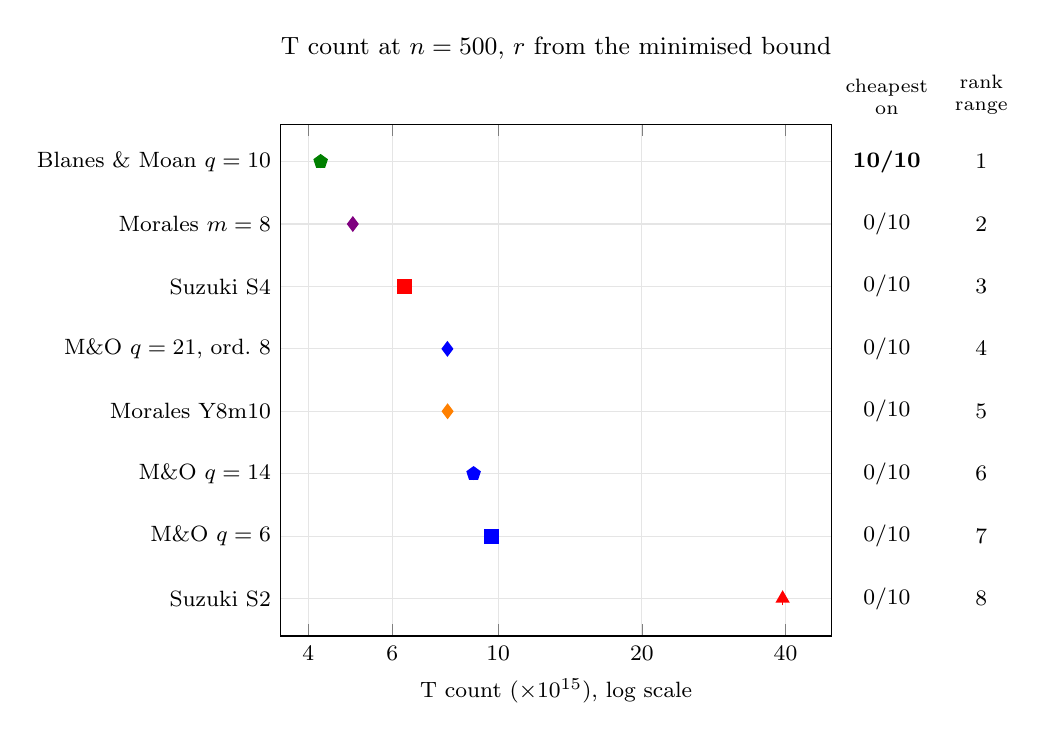
\begin{tikzpicture}
  \begin{semilogxaxis}[
    scale only axis, clip=false,
    at={(0cm,0cm)}, anchor=south west,
    width=7.0cm, height=6.5cm,
    title={T count at $n = 500$, $r$ from the minimised bound}, title style={font=\small, yshift=14pt},
    xlabel={T count ($\times 10^{15}$), log scale}, xlabel style={font=\footnotesize},
    xmin=3.5e+15, xmax=5e+16, xtick={4e+15,6e+15,1e+16,2e+16,4e+16}, xticklabels={4,6,10,20,40},
    xminorticks=false,
    y dir=reverse, ymin=0.4, ymax=8.6, ytick={1,2,3,4,5,6,7,8},
    yticklabels={{Blanes \& Moan $q=10$},{Morales $m=8$},{Suzuki S4},{M\&O $q=21$, ord.~8},{Morales Y8m10},{M\&O $q=14$},{M\&O $q=6$},{Suzuki S2}},
    tick label style={font=\footnotesize}, ytick style={draw=none},
    xmajorgrids=true, ymajorgrids=true, grid style={black!10},
  ]
    \addplot[green!50!black, only marks, mark=pentagon*, mark size=2.4pt, mark options={solid, fill=green!50!black, line width=0.6pt}, error bars/.cd, x dir=both, x explicit, error bar style={solid, line width=0.6pt}] coordinates {
      (4.24434e+15,1) += (3.04117e+11,0) -= (4.77675e+11,0)
    };
    \addplot[violet, only marks, mark=diamond*, mark size=2.4pt, mark options={solid, fill=violet, line width=0.6pt}, error bars/.cd, x dir=both, x explicit, error bar style={solid, line width=0.6pt}] coordinates {
      (4.9572e+15,2) += (2.92503e+11,0) -= (2.97895e+11,0)
    };
    \addplot[red, only marks, mark=square*, mark size=2.4pt, mark options={solid, fill=red, line width=0.6pt}, error bars/.cd, x dir=both, x explicit, error bar style={solid, line width=0.6pt}] coordinates {
      (6.36193e+15,3) += (8.36818e+11,0) -= (7.81907e+11,0)
    };
    \addplot[blue, only marks, mark=diamond*, mark size=2.4pt, mark options={solid, fill=blue, line width=0.6pt}, error bars/.cd, x dir=both, x explicit, error bar style={solid, line width=0.6pt}] coordinates {
      (7.82549e+15,4) += (7.44269e+11,0) -= (6.18116e+11,0)
    };
    \addplot[orange, only marks, mark=diamond*, mark size=2.4pt, mark options={solid, fill=orange, line width=0.6pt}, error bars/.cd, x dir=both, x explicit, error bar style={solid, line width=0.6pt}] coordinates {
      (7.83221e+15,5) += (4.54015e+11,0) -= (4.74185e+11,0)
    };
    \addplot[blue, only marks, mark=pentagon*, mark size=2.4pt, mark options={solid, fill=blue, line width=0.6pt}, error bars/.cd, x dir=both, x explicit, error bar style={solid, line width=0.6pt}] coordinates {
      (8.87764e+15,6) += (5.80449e+11,0) -= (8.95269e+11,0)
    };
    \addplot[blue, only marks, mark=square*, mark size=2.4pt, mark options={solid, fill=blue, line width=0.6pt}, error bars/.cd, x dir=both, x explicit, error bar style={solid, line width=0.6pt}] coordinates {
      (9.67956e+15,7) += (5.50269e+11,0) -= (6.70955e+11,0)
    };
    \addplot[red, only marks, mark=triangle*, mark size=2.4pt, mark options={solid, fill=red, line width=0.6pt}, error bars/.cd, x dir=both, x explicit, error bar style={solid, line width=0.6pt}] coordinates {
      (3.9433e+16,8) += (5.33124e+12,0) -= (4.16275e+12,0)
    };
    \node[anchor=south, font=\scriptsize, align=center] at ([xshift=0.7cm]axis cs:5e+16,0.4) {cheapest\\on};
    \node[anchor=south, font=\scriptsize, align=center] at ([xshift=1.9cm]axis cs:5e+16,0.4) {rank\\range};
    \node[font=\footnotesize\bfseries] at ([xshift=0.7cm]axis cs:5e+16,1) {10/10};
    \node[font=\footnotesize] at ([xshift=1.9cm]axis cs:5e+16,1) {1};
    \node[font=\footnotesize] at ([xshift=0.7cm]axis cs:5e+16,2) {0/10};
    \node[font=\footnotesize] at ([xshift=1.9cm]axis cs:5e+16,2) {2};
    \node[font=\footnotesize] at ([xshift=0.7cm]axis cs:5e+16,3) {0/10};
    \node[font=\footnotesize] at ([xshift=1.9cm]axis cs:5e+16,3) {3};
    \node[font=\footnotesize] at ([xshift=0.7cm]axis cs:5e+16,4) {0/10};
    \node[font=\footnotesize] at ([xshift=1.9cm]axis cs:5e+16,4) {4};
    \node[font=\footnotesize] at ([xshift=0.7cm]axis cs:5e+16,5) {0/10};
    \node[font=\footnotesize] at ([xshift=1.9cm]axis cs:5e+16,5) {5};
    \node[font=\footnotesize] at ([xshift=0.7cm]axis cs:5e+16,6) {0/10};
    \node[font=\footnotesize] at ([xshift=1.9cm]axis cs:5e+16,6) {6};
    \node[font=\footnotesize] at ([xshift=0.7cm]axis cs:5e+16,7) {0/10};
    \node[font=\footnotesize] at ([xshift=1.9cm]axis cs:5e+16,7) {7};
    \node[font=\footnotesize] at ([xshift=0.7cm]axis cs:5e+16,8) {0/10};
    \node[font=\footnotesize] at ([xshift=1.9cm]axis cs:5e+16,8) {8};
  \end{semilogxaxis}
\end{tikzpicture}
  \end{fitwidth}
  \caption{T count against system size, $r$ from the minimised bound: full range and $n = 200$--$500$ enlarged (top); count at $n = 500$ over seeds (bottom). $r$ from the minimised norm bound (Childs et al.\ 2018 Def.~2, extended to every formula by counting $2q$ sweeps), computed at every $n$; no fit, no extrapolation. $\epsilon = 5\times10^{-4}$ for the formula plus $5\times10^{-4}$ for synthesis; the spread ($\le 0.025\%$) comes only from synthesising each seed's field angles.}
\end{figure}
\end{document}
